\documentclass{overturerep}
%**********************************************************
%
% Bibliography support
%
%**********************************************************
%\def\@reportno{YY--NN}		% default report no.
%\def\reportno#1{\gdef\@reportno{#1}}

\newcommand{\bthisbibliography}[1]{\section*{References}%
   \begin {list} {}%
     {\settowidth {\labelwidth} {[#1]XX}%
      \setlength {\leftmargin} {\labelwidth}%
      \addtolength{\leftmargin} {\labelsep}%
      \setlength {\parsep} {1ex}%
      \setlength {\itemsep} {2ex}%
     }
  }
\newcommand{\ethisbibliography}{\end{list}}
\newcommand{\refitem}[2]
  {\bibitem[#1]{#2}}

\newcommand{\back}{$\setminus$}
\newcommand{\RuleTarget}[1]{\hypertarget{rule:#1}{}}
\newcommand{\Ruledef}[2]
{
  \RuleTarget{#1}\Rule{#1}{#2}%
  }
\newcommand{\Ruleref}[1]{
  \hyperlink{rule:#1}{#1}}
\newcommand{\Lit}[1]{`{\tt #1}\Quote}
\newcommand{\Rule}[2]{
  \begin{quote}\begin{tabbing}
    #1\index{#1}\ \ \= = \ \ \= #2  ; %    Adds production rule to index
    
  \end{tabbing}\end{quote}
  }
\newcommand{\SeqPt}[1]{\{\ #1\ \}}
\newcommand{\lfeed}{\\ \> \>}
\newcommand{\dsepl}{\ $|$\ }
\newcommand{\dsep}{\\ \> $|$ \>}
\newcommand{\Lop}[1]{`{\sf #1}\Quote}
\newcommand{\blankline}{\vspace{\baselineskip}}
\newcommand{\Brack}[1]{(\ #1\ )}
\newcommand{\nmk}{\footnotemark}
\newcommand{\ntext}[1]{\footnotetext{{\bf Note: } #1}}
\newlength{\kwlen}
\newcommand{\Keyw}[1]{\settowidth{\kwlen}{\tt #1}\makebox[\kwlen][l]{\sf
    #1}}
\newcommand{\keyw}[1]{{\sf #1}}
\newcommand{\id}[1]{{\tt #1}}
\newcommand{\metaiv}[1]{\begin{alltt}\input{#1}\end{alltt}}

\newcommand{\OptPt}[1]{[\ #1\ ]}
\newcommand{\MAP}[2]{\kw{map }#1\kw{ to }#2}
\newcommand{\INMAP}[2]{\kw{inmap }#1\kw{ to }#2}
\newcommand{\SEQ}[1]{\kw{seq of }#1}
\newcommand{\NSEQ}[1]{\kw{seq1 of }#1}
\newcommand{\SET}[1]{\kw{set of }#1}
\newcommand{\PROD}[2]{#1 * #2}
\newcommand{\TO}[2]{$#1 \To #2$}
\newcommand{\FUN}[2]{#1 \To #2}
\newcommand{\PUBLIC}{\ifthenelse{\boolean{VDMpp}}{public\mbox{}}{\mbox{}}}
\newcommand{\PRIVATE}{\ifthenelse{\boolean{VDMpp}}{private}{\mbox{}}}
\newcommand{\PROTECTED}{\ifthenelse{\boolean{VDMpp}}{protected}{\mbox{}}}

\usepackage{makeidx}

\usepackage{graphicx, color}

% definition of VDM++, JavaCC, JJTree, JTB, ANTLR and SableCC for listings
\newcommand{\NL}{\mbox{}\\ \vspace*{-5mm}}
\usepackage{listings}
\newcommand{\url}[1]{\texttt{#1}}
\usepackage{vdmsl-2e}
\usepackage{hyperref}

\usepackage{times}
\usepackage{color}
\lstdefinelanguage{VDM++}
  {morekeywords={act, active, fin, req, waiting, abs, all, allsuper, always, and, answer, 
     assumption, async, atomic, be, bool, by, card, cases, char, class, comp, compose, conc, cycles,
     dcl, def, definitions, del, dinter, div, dlmodule, do, dom, dunion, duration, effect, elems, else, elseif, end,
     error, errs, exists, exists1, exit, exports, ext, floor, for, forall, from, functions, 
     general, hd, if, imports, in, inds, infer, init, inmap, input, instance, int, inter, inv, inverse, iota, is, 
     isofbaseclass, isofclass, inv, inverse, lambda, len, let, map, measure, mu,
     mutex, mod, module, nat, nat1, new, merge, 
     munion, not, of, operations, or, others, per, periodic, post, power, pre, pref, 
     private, protected, public, qsync, rd, responsibility, return, reverse,  
     sameclass, parameters, psubset, rem, renamed, rng, sel, self, seq, seq1, set, skip, specified, st, 
     start, startlist, state, static, stop, stoplist, sporadic, subclass, subset, subtrace, sync, system, then, thread, 
     threadid, time, tixe, tl, to, token, traces, trap, types, undefined,
     union, uselib, using, values, 
     variables, while, with, wr, yet, RESULT, false, true, nil, periodic pref, rat, real},
   %keywordsprefix=mk\_,
   %keywordsprefix=a\_,
   %keywordsprefix=t\_,
   %keywordsprefix=w\_,
   sensitive,
   morecomment=[l]--,
   morestring=[b]",
   morestring=[b]',
  }[keywords,comments,strings]
\lstdefinelanguage{JavaCC}
  {morekeywords={options, PARSER\_BEGIN, PARSER\_END, SKIP, TOKEN},
   sensitive=false,
  }[keywords]

% define the layout for listings
\lstdefinestyle{tool}{basicstyle=\ttfamily,
                         frame=trBL, 
			 showstringspaces=false, 
			 frameround=ffff, 
			 framexleftmargin=0mm, 
			 framexrightmargin=0mm}
\lstdefinestyle{mystyle}{basicstyle=\footnotesize\ttfamily,
                         frame=trBL, 
%                         numbers=left, 
%			 gobble=0, 
%			 basewidth=0.51em,
                         showstringspaces=false, 
%			 linewidth=\textwidth, 
			 frameround=fttt, 
			 aboveskip=2mm,
			 belowskip=2mm,
			 framexleftmargin=0mm, 
			 framexrightmargin=0mm}
%\lstdefinestyle{mystyle}{basicstyle=\sffamily\small,
%			 frame=tb,
%                         numbers=left,
%			 gobble=0,
%			 showstringspaces=false,
%			 linewidth=345pt,
%			 frameround=ffff,
%			 framexleftmargin=8mm,
%			 framexrightmargin=8mm,
%			 framextopmargin=1mm,
%			 framexbottommargin=1mm,
%			 aboveskip=7mm,
%			 belowskip=5mm,
%			 xleftmargin=10mm,}

\lstset{style=mystyle}
\lstset{language=VDM++}
%\lstset{alsolanguage=Java}
% The command below enables you to escape into normal LaTeX mode inside your 
% VDM chunks by starting with a `!� character and ending with a `��
\lstset{escapeinside=!�}

%This file has been converted to use LaTeX2e
%\documentstyle[overture]{article}
%
% any "\include{...}" statements go here
%
\include{ifad}
\include{graphics}
\usepackage{cite}
\usepackage{alltt}
%\usepackage{fancyhdr}
\renewcommand{\topfraction}{0.9}
\renewcommand{\textfraction}{0.05}
\renewcommand{\floatpagefraction}{0.9}
\makeindex

\begin{document}
\title{User Guide for the Overture VDM Tool Support}
\author{Peter Gorm Larsen, Kenneth Lausdahl, Augusto Reibero and Sune Wolff \\ 
Engineering College of Aarhus\\
Dalgas Avenue 2, DK-8000 \AA{}rhus C, Denmark\\[3mm]
Nick Battle\\
Fujitsu Services\\
Lovelace Road, Bracknell, \\
Berkshire. RG12 8SN, UK}

\reportno{TR-2009-02}     

\maketitle

\tableofcontents

\begin{abstract}
This document is a user manual for the Overture Integrated Development
Environment (IDE) open source tool for
VDM. It can serve as a reference for anybody wishing to make use of
this tool with one of the VDM dialects (VDM-SL, VDM++ and VDM-RT).
This tool support is build of top of the Eclipse platform. The
objective of the Overture open source initiative is to enable a
platform that both can be used for experimentation of new subsets or
supersets of VDM dialects as well as new features analysing such VDM
models in different ways. The tool is entirely open source so anybody
can join the development team and influenece the future
developments. The long term target is also to ensure that stable
versions of the tool suite can be used for large scale industrial
applications of the VDM technology.
\end{abstract}

\section{Introduction}

The Vienna Development Method (VDM)is one of the longest established
model-oriented formal methods for the development of computer-based
systems and software
\cite{Bjorner&78,Jones90a,Fitzgerald&08c}. It consists of a
group of mathematically well-founded languages for expressing system
models during early design stages, before expensive implementation
commitments are made. The construction and analysis of the model using
Overture help to identify areas of incompleteness or ambiguity in
informal system specifications, and provide some level of confidence
that a valid implementation will have key properties, especially those
of safety or security. VDM has a strong record of industrial
application, in many cases by practitioners who are not specialists in
the underlying formalism or logic
\cite{Larsen&95b,Clement&99,Kurita&09}. Experience with the method
suggests that the effort expended on formal modeling and analysis can
be recovered in reduced rework costs arising from design errors.

VDM models are expressed in a specification language (VDM-SL) that
supports the description of data and functionality
\cite{ISOVDM96a,Fitzgerald&98b,Fitzgerald&09}. Data are defined by
means of types built using constructors that define structured data
and collections such as sets, sequences and mappings from basic values
such as Booleans and numbers. These types are very abstract, allowing
the user to add any relevant constraints as data type
invariants. Functionality is defined in terms of operations over these
data types. Operations can be defined implicitly by preconditions and
postconditions that characterize their behavior, or explicitly by
means of specific algorithms. An extension of VDM-SL, called VDM++,
supports object-oriented structuring of models and permits direct
modeling of concurrency \cite{Fitzgerald&05}. An additional extension
to VDM++ is called VDM Real Time (VDM-RT) (formerly called VDM In a
Constrained Environment (VICE)) \cite{Mukherjee&00,Verhoef&06b}. All
these different dialects are supported by the unified tool called Overture.

Since the VDM modeling languages have a formal mathematical semantics,
a wide range of analyses can be performed on models, both to check
internal consistency and to confirm that models have emergent
properties. Analyses may be performed by inspection, static analysis,
testing or mathematical proof. To assist in this process, Overture
supply tool support for building models in collaboration with other
modeling tools, to execute and test models and to carry out different
forms of static analysis \cite{Larsen&10a}. It can be seen as an open
source version of the commercial tool called VDMTools
\cite{Elmstrom&94,Fitzgerald&08a} although that also have features to
generate executable code in high-level programming languages which are
not yet available in Overture.

This guide explains how to use the Overture IDE for developing models
for different VDM dialects. This user manual starts with explanantion
about how to get hold of the software in
Ssection~\ref{sec:install}. This is followed in
Section~\ref{sec:vdmsupport} with an introduction to the concepts used
in the different Overture perspectives based on Eclipse
terminology. In Section~\ref{sec:projects} it is explained how
projects are managed in the Overture IDE. In Section~\ref{sec:editVDM}
the features supported when editing VDM models are explained. This is
followed in Section~\ref{sec:debug} with an explainantion of the
interpretation and debugging capabilities in the Overture
IDE. Section~\ref{sec:testcoverage} then illustates how test coverage
information can be gathered when models are interpreted. Afterwards
Section~\ref{sec:prettyprint} shows how models with and without test
coverage information can be generated to the text processing system
\LaTeX\ and automatically converted to \texttt{pdf} format if one have
\texttt{pdflatex} installed on the computer. Afterwards from
Section~\ref{sec:POmanagement} to Section~\ref{sec:showlog} different
VDM specfic features are explained. In Section~\ref{sec:POmanagement}
the use of the notion for proof obligations and its support in
Overture is explained. In Section~\ref{sec:testing} a notion of
combinatorial testing and the automation support for that in Overture
is presented. In Section~\ref{sec:vdmuml} support for mapping between
object-oriented VDM models to and from UML models is presented. In
Section~\ref{sec:ToVDMRT} it is illustrated how one can move from a
VDM++ project to a new VDM-RT project. In Section~\ref{sec:showlog} it
is shown how support to analysing and displaying logs from executing
such VDM-RT models. After these sections the main part of the user
manual is completed in Section~\ref{sec:commandline} with an
explanantion of the features from Overture that also is available from
a command-line interface.
Finally in
Appendix~\ref{sec:index} an index of significant terms used in this
user manual can be found. 


\section{Getting Hold of the Software}\label{sec:install}

The Overture project is managed on SourceForge.  The best way to run
Overture is to download a special version of Eclipse with the Overture
functionality already pre-installed. If you go to:
  \begin{quote}
  \url{http://sourceforge.net/projects/overture/files/}
  \end{quote}
  \noindent you can find
  pre-installed versions of Overture for Windows, Linux and Mac. At a
  later stage it will also be possible to use an update site to
  install it from directly in Eclipse. However, at the moment only
  stand-alone versions are distributed because the risk of version
  problems and dependencies with other plug-ins is much smaller this way.

Zip files with a large collection of existing VDM-SL, VDM++ and VDM-RT
projects can be downloaded from
\begin{quote}
\url{http://sourceforge.net/projects/overture/files/Examples/}
\end{quote}
Such existing projects can be imported as described in
subsection~\ref{subsec:importproj}. 

\section{Using the Overture Perspective}\label{sec:vdmsupport}

\subsection{Getting into the Eclipse Terminology}

Eclipse is an open source platform based around a \emph{workbench}\index{workbench} that provides
a common look and feel to a large collection of extension products. Thus if a
user is familiar with one Eclipse product, it will generally be easy to
start using a different product on the same workbench. The Eclipse workbench consists
of several panels known as \emph{views}\index{view}, such as the Script Explorer view at the
top left of Figure~\ref{fig:userguire:OverturePerspective}. A collection of
panels is called a \emph{perspective}\index{perspective}, for example
Figure~\ref{fig:userguire:OverturePerspective} shows the standard Overture
perspective. This consists of a set of views for managing Overture projects and
viewing and editing files in a project. Different perspectives are available in
Overture as will be described later, but for the moment think about a perspective as a
useful composition of views for conducting a particular task.

\begin{figure}[!h]
\begin{center}
  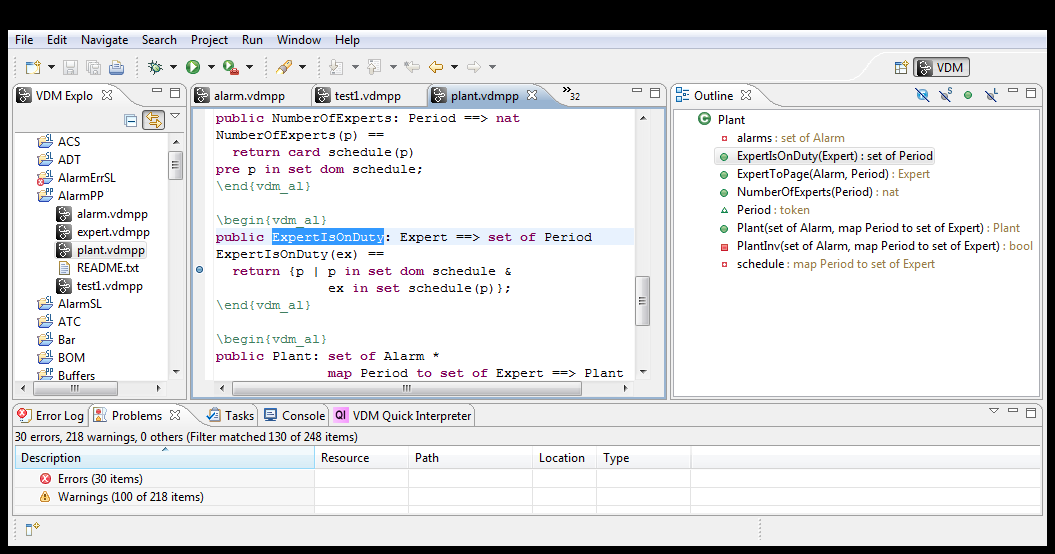
\includegraphics[width=\textwidth]{figures/OverturePerspective}
  \caption[labelInTOC]{The Overture Perspective}
  \label{fig:userguire:OverturePerspective}
\end{center}
\end{figure}

The \emph{Script Explorer view}\index{explorer} lets you create, select, and delete Overture 
projects and navigate between the files in these projects. 

Depending upon the dialect of VDM used in a given project,
a corresponding Overture editor will be available here. A new VDM-SL
project is created choosing the \emph{File} $ \rightarrow$ \emph{New}
$\rightarrow$ \emph{Project}. Then
Figure~\ref{fig:userguide:newOvertureProjectSL} will appear and \emph{Next} can
be used and then a name needs to be given to the project.


\begin{figure}[!h]
\begin{center}
  \caption[labelInTOC]{Creating a New VDM-SL Project}
  \label{fig:userguide:newOvertureProjectSL}
  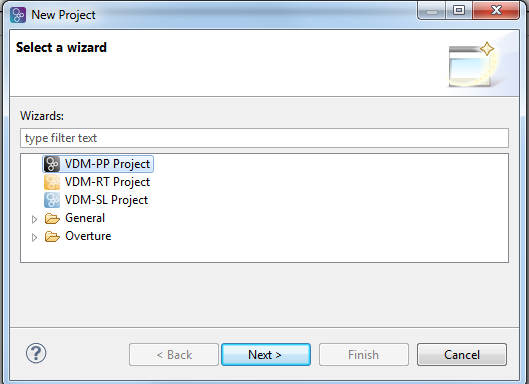
\includegraphics[width=2.5in]{figures/newovertureSLproject}
\end{center}
\end{figure}


The \emph{Outline view}\index{outline}, to the right of the editor (see
Figure~\ref{fig:userguide:OutlineView}), presents an outline of the file selected
in the editor. The outline displays any declared VDM-SL modules, as well as
their state components, values, types, functions and operations. In
case of a flat VDM-SL model the module is called {\ttfamily{DEFAULT}}.\index{DEFAULT}
% and traces.
Figure~\ref{fig:userguire:OverturePerspective} shows the outline view on the
right hand side. Clicking on an operation or function will move the cursor in
the editor to the definition of the operation. At the top of the outline view there
is a button to optionally sort what is
displayed in the outline view, for instance it is possible to hide variables.


\begin{figure}[!h]
\begin{center}
  \caption[labelInTOC]{The Outline View}
  \label{fig:userguide:OutlineView}
  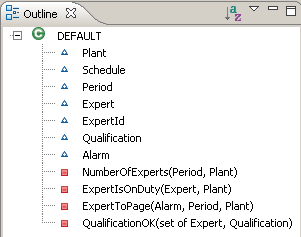
\includegraphics[width=2.5in]{figures/OutlineView}
\end{center}
\end{figure}

The \emph{Problems view}\index{problems} gathers information messages about the projects you are
working on. This includes information generated by Overture, such as
warnings and errors.

Most of the other features of the workbench, such as the menus and
toolbars, are similar to other Eclipse applications, though note that
there is a special menu with Overture specific functionality. One
convenient feature is a toolbar of shortcuts to switch between
different perspectives that appears on the right side of the screen;
these vary dynamically according to context and history.

\subsection{Additional Eclipse Features Applicable in Overture}

If one would like to use additional file types to be associated with a
particular VDM editor instead of the standard {\ttfamily vdmsl},
{\ttfamily vdmpp} and {\ttfamily vdmrt} file types this is possible in
Overture. This is done using the \emph{Window} $\rightarrow$
\emph{Preferences} menu point. Here one can start typing {\ttfamily
  contents types} and then one will get a menu similar to
Figure~\ref{fig:ContentsTypes}. Here one can press the {\ttfamily Add}
button for the appropriate contents type that one wishes to add
additional types of file extensions.\index{file extension}

\begin{figure}[!htb]
\begin{center}
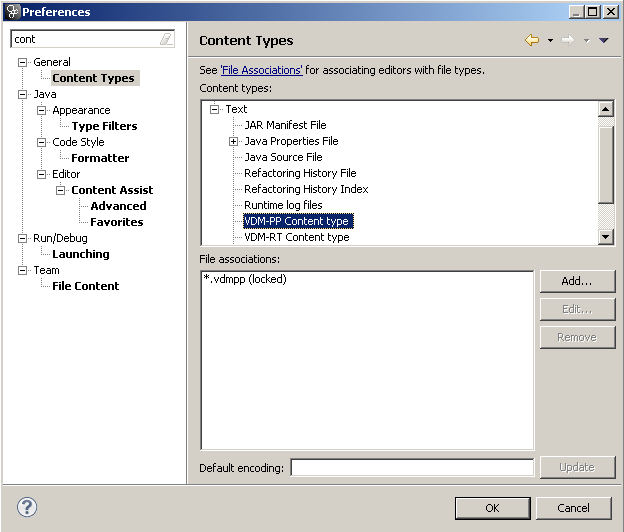
\includegraphics[width=0.6\textwidth]{screenDumps/contentstypes}
\caption{Adding Additional Contents Types\label{fig:ContentsTypes}}
\end{center}
\end{figure}

\section{Managing Overture Projects}\label{sec:projects}

\subsection{Importing Overture Projects}\label{subsec:importproj}


\subsection{Creating a New Overture Project}
\begin{enumerate}
	\item Create a new project by choosing \emph{File}
          $\rightarrow$ \emph{New} $\rightarrow$ \emph{Project}
          $\rightarrow$ \emph{Overture}; 
	\item Select the VDM dialect you wish to use (VDM-SL, VDM-PP
          or VDM-RT);\index{VDM dialect}
        \item Type in a project name
	\item Chose whether you would like the contents of the new
          project to be in your workspace or outside from existing
          source files and
        \item click
	the finish button (see \ref{fig:CreateProjectWizard}).
\end{enumerate}

\begin{figure}[!h]
	\begin{center}
	  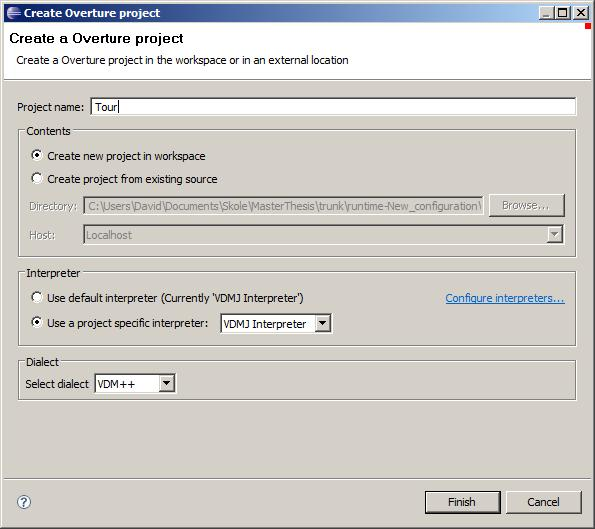
\includegraphics[scale=0.8]{figures/CreateProjectWizard}
	  \caption[Create Project Wizard]{Create Project Wizard}
	  \label{fig:CreateProjectWizard}
	\end{center}
\end{figure}

%%%%%%%%%%%%%%%%%%%%%%%%%%%%%%%%%%
%  Creating a new file
%%%%%%%%%%%%%%%%%%%%%%%%%%%%%%%%%%

\subsection{Creating Files}

Switching to the Overture perspective will change the layout of the user
interface to focus on the VDM development. To change perspective go to the menu 
window $\rightarrow$ open perspective $\rightarrow$ other\ldots and choose the
Overture perspective.
When the developer is in the Overture Perspective the user can create files
using one of the following methods:

\begin{enumerate}
  \item Choose \emph{File} $\rightarrow$ \emph{New} $\rightarrow$
    \emph{VDM-SL Module}\index{creating!VDM-SL module} or 
    \emph{VDM-PP Class}\index{creating!VDM++ class} or 
    \emph{VDM-RT Class}\index{creating!VDM-RT class} or
  \item Right click on the Overture project where you would like to
    add a new file and then choose \emph{New} $\rightarrow$ $\rightarrow$
    \emph{VDM-SL Module} or \emph{VDM-PP Class} or \emph{VDM-RT Class}.
\end{enumerate}

In both cases one needs to choose a file name and optionally choose a
directory if one does not want to place the file in the directory for
the chosen Overture project. Then a new file with the appropriate file
extension according to the chosen dialect (\texttt{vdmsl},
\texttt{vdmpp} or \texttt{vdmrt})\index{vdm file extension} can be
created in the selected directory. This file will use the appropriate
module/class template to get the user started with defining the
module/class meant to be placed in this new file. Naturally keywords
for kinds of definitions that will not be used can be deleted.

\subsection{Setting Project Options}\label{subsec:options}


\section{Editing VDM models}\label{sec:editVDM}


\section{Interpretation and Debugging in Overture}\label{sec:debug}

This section describes how to debug a model using the Overture IDE. 

\subsection{Debug configuration}

Debugging the model under development is done by creating a debug configuration
\index{debug configuration}
from the menu \emph{Run} $\rightarrow $ \emph{Debug configuration}
\ldots 
The debug
configuration dialog requires the following information as input to start the
debugger: the project name, the class, the starting operation/function and the
file containing the starting operation/function.
Figure~\ref{fig:userguide:debugConfiguration} shows a debug configuration,
clicking one of the browse buttons will open a dialog which give the user a list
of choices. The class and operation/function are chosen from the dialog with the
list of expandable classes, if the operation or function have arguments these
must be typed in manually.

\begin{figure}[htp]
\begin{center}
  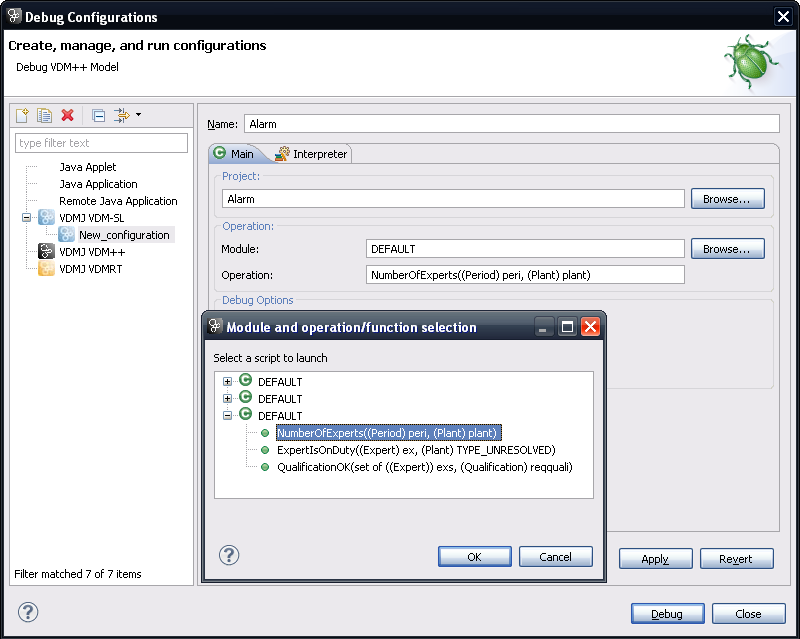
\includegraphics[width=380px]{figures/debugConfiguration}
  \caption{The debug configuration dialog}
  \label{fig:userguide:debugConfiguration}
\end{center}
\end{figure}

\subsection{Debug Perspective}

The Debug Perspective\index{debug perspective} contains the views
needed for debugging in VDM. Breakpoints can easily be set at desired
places in the model, by double clicking in left margin. When the
debugger reaches the location of the breakpoint, the user can inspect
the values of different identifiers and step through the VDM model
line by line.
 
The debug perspective shows the VDM model in an editor as the one used in the
Overture Perspective, but in this perspective there are also views useful during
debugging. The features provided in the debug perspective are described below.
The Debug Perspective is illustrated on figure~\ref{fig:userguide:DebuggingVDM}

\begin{figure}[htp]
\begin{center}
  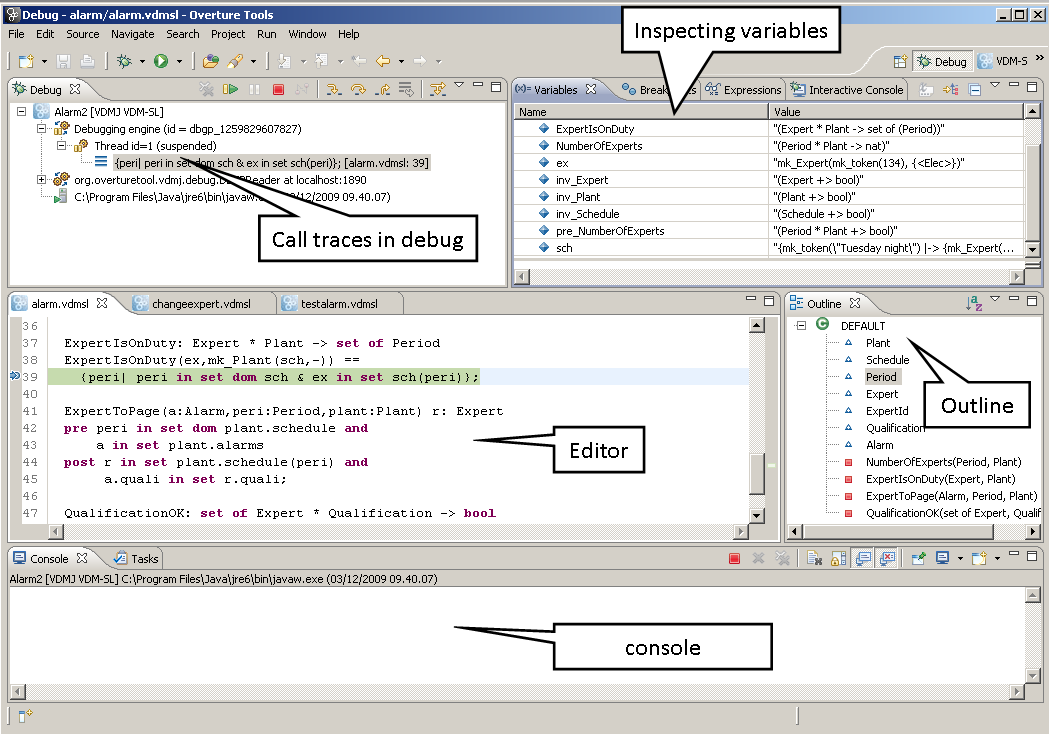
\includegraphics[width=380px]{figures/DebuggingVDM}
  \caption[Debugging perspective]{Debugging perspective}
  \label{fig:userguide:DebuggingVDM}
\end{center}
\end{figure}

The \emph{Debug view} is located in the upper left corner in the Debug
perspective. The Debug view shows all running models and the call stacks
belonging to them. It also shows whether a given model is stopped, suspended or
running. All threads are also shown, along with their running status. It is
possible to switch between threads from the Debug view.

\begin{table}
\begin{center}
\caption{Overture debugging buttons\label{tab:debugButtons}}
\begin{tabular}{|l|l|}\hline \hline
\textbf{Button} & \textbf{Explanation} \\ \hline

\includegraphics[width=0.06\textwidth]{figures/resume} & Resume
debugging\index{icon!resume debugging} \\

\includegraphics[width=0.06\textwidth]{figures/suspend} & Suspend
debugging\index{icon!suspend debugging}\\

\includegraphics[width=0.06\textwidth]{figures/terminate} & Terminate
debugging\index{icon!terminate debugging}\\

\includegraphics[width=0.06\textwidth]{figures/stepinto} & Step
into\index{icon!step into}\\

\includegraphics[width=0.06\textwidth]{figures/stepover} & Step
over\index{icon!step over} \\

\includegraphics[width=0.06\textwidth]{figures/stepreturn} & Step
return\index{icon!step return}\\

\includegraphics[width=0.06\textwidth]{figures/stepbystep} & Use step
filters\index{icon!use step filters}\\
\hline \hline
\end{tabular}
\end{center}
\end{table}

At the top of the view are buttons for controlling debugging such as; stop, step
into, step over and resume. These are standard Eclipse debugging
buttons (see Table~\ref{tab:debugButtons}).


\subsubsection{Debug View}

The debug View is located in the upper left corner in the Debug Perspective -
see figure \ref{fig:userguide:DebuggingVDM}. The debug view shows all running
models and the call stack belonging to them. It also displays whether a given model is
stopped, suspended or running. In the top of the view buttons
for debugging such as; stop, step into, step over, resume, etc.\ are located.
All threads are also shown, along with their running status. It is possible to
switch between threads from the Debug View.

\subsubsection{Variables View}
 
This view shows all the variables in a given context, when a breakpoint is
reached. The variables and their values displayed are automatically updated when
stepping through a model. The variables view is by default located in the upper
right hand corner in the Debug Perspective. It is also possible to inspect complex variables,
expanding nested arrays and so forth.

\subsubsection{Breakpoints View}

Breakpoints can be added both from the edit perspective and the debug perspective
from the editor view. In the debug perspective however, there is a breakpoints
view that shows all breakpoints. From the breakpoints view the user can easily
navigate to the location of a given breakpoint, disable, delete or set the hit
count or a break condition. In figure \ref{fig:userguide:DebuggingVDM} the
Breakpoints View is hidden behind the Variables View in the upper right hand 
corner in a tabbed notebook. Section~\ref{sec:userguide:breakpoints} explains
how to use conditional breakpoints.

\subsubsection{Expressions View}

The expressions view allows the user to write expressions, as for the
variables view, the expressions are automatically updated when stepping.
Watch expressions can be added manually or created by selecting 'create watch
expression' from the variables view. It is of course possible to edit existing
expressions. Like the Breakpoints View this view is hidden in the upper right
hand corner.

\subsubsection{Interactive Console View}

While the Expressions View allows to easily inspect values, the functionality is
somewhat limited compared with the functionality provided by VDMTools. For more
thorough inspections the Interactive Console View is more suited. Here commands
can be executed on the given context, i.e.\ where the debugger is at a
breakpoint. The Interactive console keeps a command history, so that already
executed commands can be run again without actually typing in the command all
over. Figure~\ref{fig:userguide:interactiveConsole} shows the interactive
console.

\begin{figure}[htp]
\begin{center}
  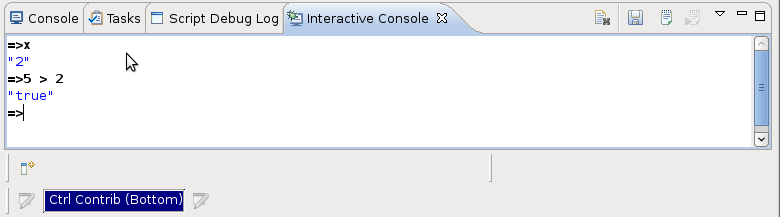
\includegraphics[width=300px]{figures/InteractiveConsole}
  \caption{The interactive console}
  \label{fig:userguide:interactiveConsole}
\end{center}
\end{figure}

\subsubsection{Conditional breakpoints}
\label{sec:userguide:breakpoints}

Conditional breakpoints can also be defined. These are a powerful tool for the
developer since it allows specifying a condition for one or more variables which
has to be true in order for the debugger to stop at the given breakpoint. Apart
from specifying a break condition depending on variables, a hit count can also be
defined. A conditional breakpoint with a hit count lets the user specify a given
number of calls to a particular place at which the debugger should break.

Making a breakpoint conditional is done by right clicking on the breakpoint
mark in the left margin and select the option Breakpoint properties\ldots This
opens a dialog like the one shown in
figure~\ref{fig:userguide:BreakpointConditional}. It is possible to choose
between two different conditional breakpoints, a hit count condition and one
based on an expression defined by the user. 

\begin{figure}[htp]
\begin{center}
  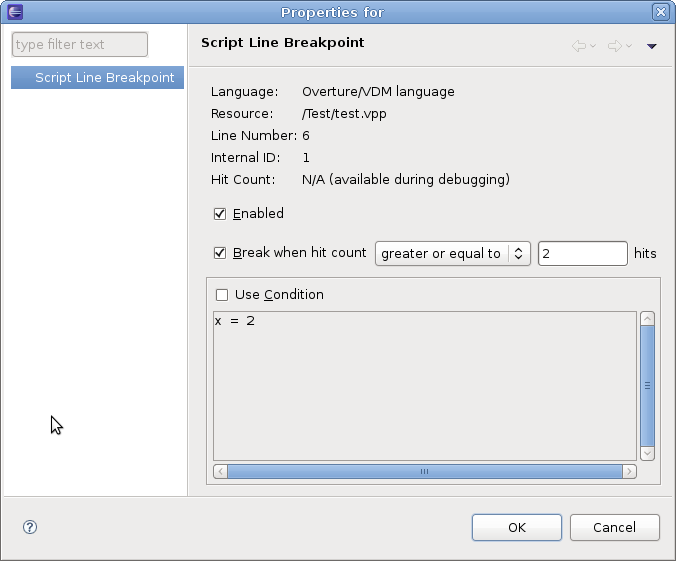
\includegraphics[width=250px]{figures/Breakpointconditional}
  \caption{Conditional breakpoint options}
  \label{fig:userguide:BreakpointConditional}
\end{center}
\end{figure}

\section{Collecting Test Coverage Information}\label{sec:testcoverage}

When a VDM model is being interpreted it is possible to automatically
collect test coverage information. 
Test coverage measurement helps you to see
how well a given test suite\index{Test Coverage!Test suite} covers the
VDM model. This is done by collecting information in a special
test coverage file about which statements and expressions are
evaluated during the execution of the test suite.

\section{Pretty Printing to \LaTeX}\label{sec:prettyprint}

Include {\ttfamily overture.tex} which among other things makes use of
the {\ttfamily times.cls} and {\ttfamily listings.cls} style
classes. This emables the use of the standard {\ttfamily lstlisting}
environment for type setting source text and display it in a tele-type
proportional font where all VDM keyword are typeset in a bold
font. Per default the listings will be inserted into boxes but it is
easy to adjust (using the parameters to the {\ttfamily lstlisting}
environment) if no boxes are desired.

It is possible to use literate programming/specification
\cite{Johnson96} just as inside VDMTools. Then one needs to use the
\LaTeX\ text processing system with plain VDM models mixed with
textual documentation.  The 
VDM model parts must be enclosed within ``\verb+\begin{vdm_al}+''
and ``\verb+\end{vdm_al}+''. The text-parts outside the specification
blocks are ignored by the parser (but used by the pretty-printer).

\section{Managing Proof Obligations}\label{sec:POmanagement}

In the different VDM dialects it is possible to identify places where
run-time errors potentially could occur if the model was to be
executed. In essence these can be considered as additional to the
existing type checking performed. Just like almost all other computer
based languages it is not possible to automatically statically check
if such places indeed could result in a run-time error or not. Thus
Overture provides socalled ``proof obligations''\index{proof
  obligation} for all places where such run-time errors ``could''
occur. Each \emph{Proof Obligation} (PO) is formulated as a predicate
that must hold on a particular place of the VDM model and thus it may
have particular context information associated with it. These POs can
be considered as constraints that will gurantee the internal integrity
of the VDM models if they are all correct. In the long term it will be
possible to prove these constraints by a proof component in Overture
but this is not yet working as well as we wish. 

It takes a little time for newcommers to VDM to get used to the form
of these so it may be worthwhile to elaborate a bit on the form of the
proof obligations. Theses can be divided into different
categories\index{proof obligation!categories}
depending upon their nature. These can be found in
Appendix~\ref{app:POcategories} along with a small explanation for
each of them.

The proof obligation generator is invoked either on a VDM project (and
then POs for all the VDM model files will be generated) or for a
selected VDM file one can right click in the \emph{Explorer} view and
then select the \emph{Proof Obligations} $\rightarrow$ \emph{Generate Proof
  Obligations} menu item. Overture will then change into a special
\emph{Proof Obligations Perspective}\index{proof
  obligation!perspective} as shown in Figure~\ref{fig:POview}.  

\begin{figure}[htbp]
\begin{center}
%\includegraphics[width=4.5in]{figures/POview}
\caption{The Proof Obligation perspective\label{fig:POview}}
\end{center}
\end{figure}

\section{Combinatorial Testing}\label{sec:testing}

In order to automate parts of the testing process a notion of
\emph{traces} have been introduced into VDM++ (note that this is not
yet available for VDM-SL models). Such traces conceptually correspond
to regular expressions that can be expanded to a collection of test
cases. Each such test case is then composed as a sequence of operation
calls. If a user defines such traces it is possible to make use of a
special combinatorial testing perspective that enables the automatic
unfolding of the traces and automatic execution of each of the test
cases. Subsequently the results of running all these can be inspected
and test cases that have detected errors in the VDM++ model can easily
be found and the user can then fix the problem and reuse the same
traces definitions.

\subsection{The Use of the Trace Definition Syntax}\label{sec:syntax}

The syntax for trace definitions are defined as:

\Rule{traces definitions}{\Lop{traces},
   \SeqPt{\Ruleref{named trace}}
}

\Rule{named trace}{\Ruleref{identifier},
  \SeqPt{\Lit{/}, \Ruleref{identifier}},
  \Lit{:},\Ruleref{trace definition list}
}

The naming of trace definitions (with the ``\texttt{/}'' separator) 
is used for indicating the paths
that are used for generated argument files for test cases
(\texttt{.arg}) and the corresponding result files
(\texttt{.res})\footnote{Currently the full path names are however
  not supported in an Overture context but this is envisaged in the future.}.

\Rule{trace definition list}{
  \Ruleref{trace definition term}, 
  \SeqPt{\Lit{;}, \Ruleref{trace definition term}}
}

So the ``\texttt{;}'' operator is used for indicating a sequencing
relationship between its \emph{trace definition term}'s.

\Rule{trace definition term}{
  \Ruleref{trace definition} \dsep
  \Ruleref{trace definition term}, \Lit{|}, \Ruleref{trace definition}
}

So the ``\texttt{|}'' operator is used for indicating alternative
choices between trace definitions. 

\Rule{trace definition}{
  \Ruleref{trace core definition} \dsep
  \Ruleref{trace bindings}, \Ruleref{trace core definition} \dsep
  \Ruleref{trace core definition}, \Ruleref{trace repeat pattern} \dsep
  \Ruleref{trace bindings}, \Ruleref{trace core definition}, 
  \Ruleref{trace repeat pattern}
}

Trace definitions can have different forms and combinations:

\begin{itemize}
\item Core definitions which includes application of operations and
  bracketed trace expressions.
\item Trace bindings where identifiers can be bound to values and in
  case of looseness ({\bf\ttfamily let} \emph{bind} {\bf\ttfamily in
  set} \emph{setexpr} {\bf\ttfamily in} \emph{expr}) this will
  give raise to multiple test cases generated.
\item Trace repeat patterns which are used whenever repetition is
  desired.
\end{itemize}

\Rule{trace core definition}{
  \Ruleref{trace apply expression} \dsep
  \Ruleref{trace bracketed expression}
}

\Rule{trace apply expression}{
  \Ruleref{identifier}, \Lit{.}, \Ruleref{identifier}, 
  \Lit{(}, \Ruleref{expression list}, \Lit{)}
}

Trace apply expressions are the most basic element in trace
definitions. The identifier before the ``\texttt{.}'' indicate an
object for with the operation (listed after the ``\texttt{.}'') is to
be applied with a list of arguments (the expression list inside the
brackets). Note that with the current syntax for trace definitions
apply expressions are limited to this form \texttt{instid.opid(args)} so it
is for example not at the moment possible to call an operation in the
same class directly as \texttt{opid(args)}. Nor is it possible with the
current syntax to make use of a particular operation in a superclass
in case of multiple possible ones which in VDM++ is would be written
as \texttt{instid.clid`opid(args)}. In the current version it is also
not allowed to call functions here directly, although that may be
changed at some stage in the future.

\Rule{trace repeat pattern}{
  \Lit{*} \dsep 
  \Lit{+} \dsep
  \Lit{?} \dsep
  \Lit{\{}, \Ruleref{numeric literal}, \Lit{\}} \dsep
  \Lit{\{}, \Ruleref{numeric literal}, \Lit{,} 
  \Ruleref{numeric literal}, \Lit{\}}
} 

The different kinds of repeat patterns have the following meanings:
\begin{itemize}
\item  \Lit{*} means 0 to n occurrences (n is tool specific). 
\item  \Lit{+} means 1 to n occurrences (n is tool specific). 
\item  \Lit{?} means 0 or 1 occurrences. 
\item  \Lit{\{}, n, \Lit{\}} means n occurrences.
\item  \Lit{\{}, n, \Lit{,} m \Lit{\}} means between n and m occurrences.
\end{itemize}

\Rule{trace bracketed expression}{
  \Lit{(}, \Ruleref{trace definition list}, \Lit{)}
}

\Rule{trace bindings}{
  \Ruleref{trace binding}, \SeqPt{\Ruleref{trace binding}}
}

\Rule{trace binding}{
  \Lop{let}, \Ruleref{local definitions}, 
             \SeqPt{\Lit{,}, \Ruleref{local definition}}, \Lop{in} \dsep
  \Lop{let}, \Ruleref{bind}, \Lop{in} \dsep
  \Lop{let}, \Ruleref{bind}, \Lop{be}, \Lop{st}, \Ruleref{expression}, \Lop{in}
}

\subsection{Using the Combinatorial Testing GUI}

Different icons are used to illustrate the verdict in a test
case. These are:
\begin{description}
\item[\hspace{-1.8mm}
\raisebox{-0.8mm}{
\includegraphics[width=0.03\textwidth]{icons/unknownWhiteBG.png}}:]
  This icon is used to indicate that the test case has not yet been
  executed.
\index{icon!not yet executed}
\item[\hspace{-1.8mm}
\raisebox{-0.8mm}{
\includegraphics[width=0.03\textwidth]{icons/okBigWhiteBG.png}}:] This icon is used to indicate that the test case has a pass
  verdict.\index{icon!pass verdict}
\item[\hspace{-1.8mm}
\raisebox{-0.8mm}{
\includegraphics[width=0.03\textwidth]{icons/undeterminedBigWhiteBG.png}}:] This icon is used to indicate that the test case has an inconclusive
  verdict.\index{icon!inconclusive verdict}
\item[\hspace{-1.8mm}
\raisebox{-0.8mm}{
\includegraphics[width=0.03\textwidth]{icons/faildBigWhiteBG.png}}:]
This icon is used to indicate that the test case has a fail
verdict.\index{icon!fail verdict}
\item[\hspace{-1.8mm}
\raisebox{-0.8mm}{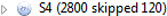
\includegraphics[height=10pt]{screenDumps/skippedIndication.png}}:] 
If test cases result in a run-time error other test cases with the
same prefix will be filtered away and thereby skipped by in the test
execution. The number of skipped test cases is indicated after number
of test cases for the trace definition name.\index{icon!skipped test case}
\end{description}

\section{Mapping VDM++ back and forth to UML}\label{sec:vdmuml}

For VDM++ projects (and later on also for VDM-RT projects) it is
possible automatically to move back and forth between a VDM++ model
and its corresponding UML model. Essentially these can be considered
as different views of the same model. The UML model is typically used
as a graphical overview of the model using class diagrams and the
sequence diagrams can be used to indicate the desired test scenarios
that a user would like to perform. The VDM++ model is typically used
as the model where the details for each definition can be found and
used for detailed semantic analysis. The exchange between VDM++ and
UML is done using the XML formal called XMI\index{XMI}. At the moment
only the UML tool Enterprise Architect\index{Exterprise Architect} is
supported. 

Mapping back and firth between a VDM++ model and a UML model is in
practice done from the \emph{Explorer} view where right-clicking on
the project will result in a menu popping up. In this menu there is an
entry for \emph{UML transformation}\index{UML transformation}. If this
is selected it is either possible to \emph{Import XMI}\index{import
  XMI} if one wish to import UML definitions from UML or to
\emph{Export XMI}\index{Export XMI} if one wish to go from VDM++ to
UML.

\section{Moving from VDM++ to VDM-RT}\label{sec:ToVDMRT}

In the methodology for the development of distributed real-time
embedded systems using the VDM techniology there is a step where one
moves from a VDM++ model to a VDM-RT model \cite{Larsen&09b}. This
step is supported by the Overture tool suite where it is possible to
copy a VDM++ project into the starting point for a VDM-RT
project. This is done by right clicking on the VDM++ project to be
converted in this fashion in the Project Explorer view. In the menu
that comes up one then need to select the \emph{Overture Utility}
$\rightarrow$ \emph{Create Real Time Project}.\index{create real time
  project} As a consequence a new VDM-RT project is
created.\index{create!VDM-RT project} It will be called exactly the
same as the VDM++ project with \texttt{RT} appended to the project
name. Inside the project all the \texttt{vdmpp} files will instead
have the \texttt{vdmrt} extension. The original VDM++ project is not
changed at all. Thus this is simply an easy way to fast get the
starting point for a VDM-RT model developed. One then manually need to
create a {\ttfamily\bf system} with appropriate declarations of
\texttt{CPU}s and \texttt{BUS}ses.
 
\section{Analysing and Displaying Logs from VDM-RT Executions}\label{sec:showlog}
When a VDM-RT model is being executed a textual logfile is created in
a ''logs/debugconfig'' folder with the \emph{.logrt} extension. The
file name for the logfile indicates the time at which it has been
written so it is possible to store multiple of these. This logfile can be
viewed in the build-in RealTime Log Viewer,\index{RealTime Log viewer}
by double-clicking the file in the project view. The viewer enables
the user to explore system execution in various perspectives. In
Figure~\ref{fig:userguide:ArchitecturalOverview} the architectural
overview of the system is given, describing the distributed nature of
the model.\index{architecture overview}

\begin{figure}[htp]
\begin{center}
  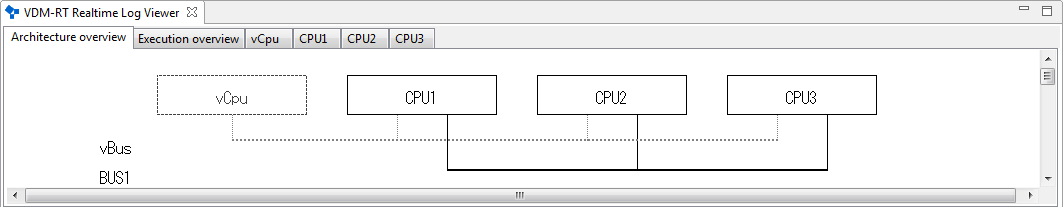
\includegraphics[width=4in]{figures/ArchitectureOverview}
  \caption{Architectural overview}
  \label{fig:userguide:ArchitecturalOverview}
\end{center}
\end{figure}

The RealTime Log Viewer also enables the user to get an overview of
the model execution\index{model execution overview} on a system level -- this can be seen in
Figure~\ref{fig:userguide:ExecutionOverview}. This view shows how the
different CPUs\index{CPU} communicate via the BUSes\index{BUS} of the system. 

\begin{figure}[htp]
\begin{center}
  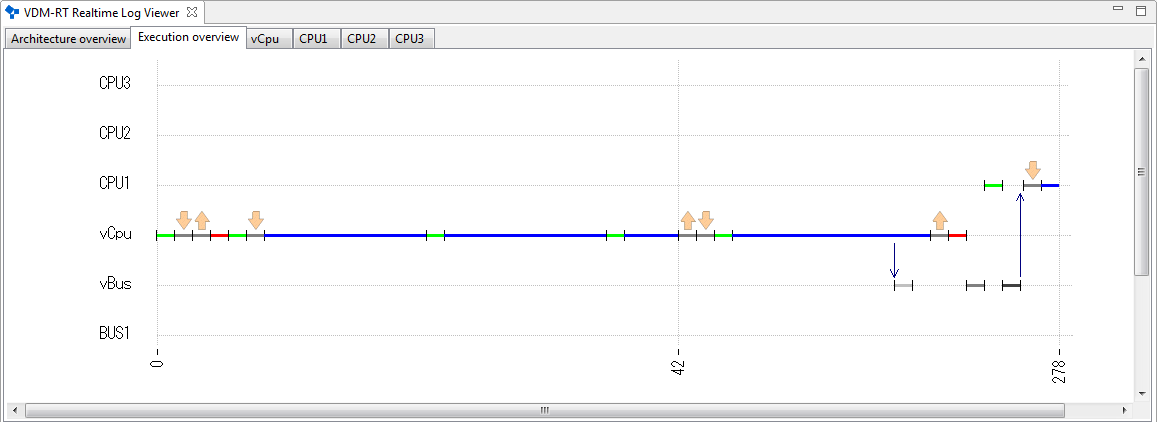
\includegraphics[width=4in]{figures/ExecutionOverview}
  \caption{Execution overview}
  \label{fig:userguide:ExecutionOverview}
\end{center}
\end{figure}

Since the complete execution of the model cannot be shown in a normal
sized window, the user has the option of jumping the a certain time
using the \emph{Go to time} button.\index{Go to time button} It is
also possible to export all the generated views to \emph{JPG} format
using the \emph{Export Image} button.\index{export image button} All
the generated pictures will be placed in the ''logs'' folder.

In addition to the execution overview, the RealTime Log Viewer can
also give an overview of all executions on a single CPU. This view
gives a detailed description of all operations and functions invoked
on the CPU as well as the scheduling of concurrent processes. This can
be seen in Figure~\ref{fig:userguide:ExecutionCPU}.\index{single CPU overview} 

\begin{figure}[htp]
\begin{center}
  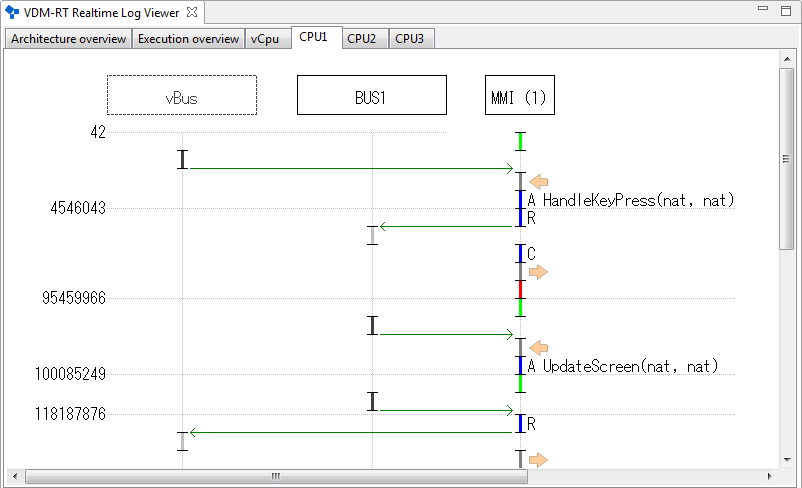
\includegraphics[width=4in]{figures/ExecutionCPU}
  \caption{Execution on single CPU}
  \label{fig:userguide:ExecutionCPU}
\end{center}
\end{figure}

\section{A Command-Line Interface to VDMJ}\label{sec:commandline}

A central part of the Overture tool is gathered in a java application
called VDMJ that enables a command-line interface that may be valuable
for users outside the Eclipse interface of Overture.

\subsection{Starting VDMJ}

VDMJ\index{VDMJ} is contained entirely within one jar file. The jar
file contains a MANIFEST that identifies the main class to start the
tool, so the minimum command line invocation is as follows:

\lstset{style=tool,language=}
\begin{lstlisting}
$ !\textbf{java -jar vdmj-2.0.0.jar}�
VDMJ: You must specify either -vdmsl, -vdmpp or -vdmrt
Usage: VDMJ <-vdmsl | -vdmpp | -vdmrt > [<options>] [<files>]
-vdmsl: parse files as VDM-SL
-vdmpp: parse files as VDM++
-vdmrt: parse files as VICE
-w: suppress warning messages
-q: suppress information messages
-i: run the interpreter if successfully type checked
-p: generate proof obligations and stop
-e <exp>: evaluate <exp> and stop
-c <charset>: select a file charset
-t <charset>: select a console charset
-o <filename>: saved type checked specification
-pre: disable precondition checks
-post: disable postcondition checks
-inv: disable type/state invariant checks
-dtc: disable all dynamic type checking
-log: enable real-time event logging
\end{lstlisting}
\lstset{style=mystyle}
\lstset{language=VDM++}

Notice that the error indicates that the tool must be invoked with either the \texttt{-vdmsl}, \texttt{-vdmpp} or \texttt{-vdmrt}
option to indicate the VDM dialect and parser required.

Normally, a specification will be loaded by identifying all of the VDM source files to include. At least
one source file must be specified unless the -i option is used, in which case the interpreter can be
started with no specification.

If no \texttt{-i} option is given, the tool will parse and type check
the specification files only, giving any errors and warnings on
standard output, then stop. Warnings can be suppressed with the \texttt{-w}
option. The \texttt{-q} option can be used to suppress the various
information messages printed (this does not include errors and
warnings).

The \texttt{-p} option will run the proof obligation generator and
then stop, assuming the specification has no type checking errors.
For batch execution, the \texttt{-e} option can be used to identify a
single expression to evaluate in the context of the loaded
specification, assuming the specification has no type checking errors.

The \texttt{-c} and \texttt{-t} options allow the file and console character sets to be defined, respectively. This is to
allow a specification written in languages other than the default for your system to be used (see
section 3).

The \texttt{-o} option allows a parsed and type checked specification to be saved to a file. Such files are
effectively libraries, and can be can be re-loaded without the parsing/checking overhead.
The \texttt{-pre}, \texttt{-post}, \texttt{-inv} and \texttt{-dtc} options can be used to disable precondition, postcondition, invariant and
dynamic type checking, respectively. By default, all these checks are performed.
The \texttt{-log} option is for use with \texttt{-vdmrt}, and causes real-time events from the model to be written to the
file name given. These are useful with the Overture Eclipse GUI, which has a plugin to display timing
diagrams [8].

If flat.vdmsl contains a simple VDM-SL specification of the factorial
function, called ``\texttt{fac}'', the following
illustrate ways to test the specification, with user input shown in bold:

\begin{lstlisting}
functions
fac: int -> int
fac(a) == if a < 2 then 1 else a * fac(a-1)
pre a > 0
\end{lstlisting}
\lstset{style=tool,language=}

\begin{lstlisting}
$ !\textbf{java -jar vdmj-2.0.0.jar -vdmsl flat.vdmsl}�
Parsed 1 module in 0.202 secs. No syntax errors
Warning 5012: Recursive function has no measure in (flat.vdmsl) at 
line 3:1
Type checked 1 module in 0.016 secs. No type errors and 1 warning
\end{lstlisting}

\begin{lstlisting}
$ !\textbf{java -jar vdmj-2.0.0.jar -vdmsl -q -w flat.vdmsl}�
<quiet!>
\end{lstlisting}

\begin{lstlisting}
$ !\textbf{java -jar vdmj-2.0.0.jar -vdmsl -w -e "fac(10)" flat.vdmsl}�
Parsed 1 module in 0.28 secs. No syntax errors
Type checked 1 module in 0.031 secs. No type errors, 
suppressed 1 warning
Initialized 1 module in 0.031 secs.
3628800
Bye
\end{lstlisting}

\begin{lstlisting}
$ !\textbf{java -jar vdmj-2.0.0.jar -vdmsl -e "fac(10)" -q -w flat.vdmsl}�
3628800
\end{lstlisting}

\begin{lstlisting}
$ !\textbf{java -jar vdmj-2.0.0.jar -vdmsl -i -w flat.vdmsl}�
Parsed 1 module in 0.202 secs. No syntax errors
Type checked 1 module in 0.016 secs. No type errors, 
suppressed 1 warning
Initialized 1 module in 0.031 secs.
Interpreter started
> !\textbf{print fac(10)}�
= 3628800
Executed in 0.0 secs.
> !\textbf{quit}�
Bye
\end{lstlisting}

\begin{lstlisting}
$ !\textbf{java -jar vdmj-2.0.0.jar -vdmsl -p -w flat.vdmsl}�
Parsed 1 module in 0.218 secs. No syntax errors
Type checked 1 module in 0.015 secs. No type errors, 
suppressed 1 warning
Generated 1 proof obligation:
Proof Obligation 1:
fac: function apply obligation in 'DEFAULT1' (flat.vdmsl) at 
line 4:38
(forall a:int & (a > 0) =>
(not (a < 2) =>
pre_f((a - 1))))
\end{lstlisting}

\begin{lstlisting}
$ !\textbf{java -jar vdmj-2.0.0.jar -vdmsl -w -e "fac(0)" -w flat.vdmsl}�
Parsed 1 module in 0.203 secs. No syntax errors
Type checked 1 module in 0.015 secs. No type errors, 
suppressed 1 warning
Initialized 1 module in 0.016 secs.
Execution: Error 4055: Precondition failure: pre_f in (flat.vdmsl) 
at line 5:11
   a = 0
   fac = (int -> int)
   pre_fac = (int +> bool)
In root context of fac(a) in 'DEFAULT1' (console) at line 1:1
In root context of interpreter in 'DEFAULT1' (flat.vdmsl) at 
line 3:1
In root context of global environment
Bye
\end{lstlisting}

\begin{lstlisting}
$ !\textbf{java -jar vdmj-2.0.0.jar -vdmsl -w -pre -e "fac(0)" 
-w flat.vdmsl}�
Parsed 1 module in 0.218 secs. No syntax errors
Type checked 1 module in 0.016 secs. No type errors, 
suppressed 1 warning
Initialized 1 module in 0.015 secs.
1
Bye
\end{lstlisting}

\begin{lstlisting}
$ !\textbf{java -jar vdmj-2.0.0.jar -vdmsl -w -o flat.lib flat.vdmsl}�
Parsed 1 module in 0.203 secs. No syntax errors
Type checked 1 module in 0.016 secs. No type errors, 
suppressed 1 warning
Saved 1 module to flat.lib in 0.093 secs.
\end{lstlisting}

\begin{lstlisting}
$ !\textbf{java -jar vdmj-2.0.0.jar -vdmsl flat.lib -e "fac(10)"}�
Loaded 1 module from flat.lib in 0.187 secs
Initialized 1 module in 0.0 secs.
3628800
Bye
\end{lstlisting}

\subsection{Parsing, Type Checking, and Proof Obligations}

All specification files loaded by VDMJ are parsed and type checked
automatically. There are no type checking options; the type checker
always uses ``possible'' semantics. If a specification does not parse
and type check cleanly, the interpreter cannot be started and proof
obligations cannot be generated (though warnings are allowed).

All warnings and error messages are printed on standard output, even
with the \texttt{-q} option.  A source file may contain VDM embedded
in a LaTeX file; the markup is ignored by the parser, though reported
line numbers will be correct.

The Java program will return with an exit code of zero if the
specification is clean (ignoring warnings).  Parser or type checking
errors result in an exit code of 1. The interpreter and PO generator
always exit with a code of zero.

\subsection{The Interpreter}

Assuming a specification does not contain any parse or type checking errors, the interpreter can be
started by using the \texttt{-i} command line option.
The interpreter is an interactive command line tool that allows expressions to be evaluated in the
context of the specification loaded. The interpreter prompt is ``\texttt{>}''. The following illustrates some of the
interactive interpreter commands (explanation below. The shmem source
model is in Appendix A):

\begin{lstlisting}
$ !\textbf{java -jar vdmj-2.0.0.jar -vdmsl -i shmem.vdmsl}�
Parsed 1 module in 0.266 secs. No syntax errors
Type checked in 0.047 secs. No type errors
Interpreter started
\end{lstlisting}

\begin{lstlisting}
> !\textbf{help}�
modules - list the loaded module names
default <module> - set the default module name
state - show the default module state
print <expression> - evaluate expression
assert <file> - run assertions from a file
init - re-initialize the global environment
env - list the global symbols in the default environment
pog - generate a list of proof obligations
break [<file>:]<line#> [<condition>] - create a breakpoint
break <function/operation> [<condition>] - create a breakpoint
trace [<file>:]<line#> [<exp>] - create a tracepoint
trace <function/operation> [<exp>] - create a tracepoint
remove <breakpoint#> - remove a trace/breakpoint
list - list breakpoints
coverage [<file>|clear] - display/clear file line coverage
latex|latexdoc [<files>] - generate LaTeX line coverage files
files - list files in the current specification
reload - reload the current specification files
load <files> - replace current loaded specification files
quit - leave the interpreter
\end{lstlisting}

\begin{lstlisting}
> !\textbf{modules}�
M (default)
\end{lstlisting}

\begin{lstlisting}
> !\textbf{state}�
M`Q4 = [mk_M(<FREE>, 0, 9999)]
M`rseed = 87654321
M`Memory = mk_Memory(87654321, [mk_M(<FREE>, 0, 9999)],
                               [mk_M(<FREE>, 0, 9999)])
M`Q3 = [mk_M(<FREE>, 0, 9999)]
\end{lstlisting}

\begin{lstlisting}
> !\textbf{print rand(100)}�
= 71
Executed in 0.0 secs.
\end{lstlisting}

\begin{lstlisting}
> !\textbf{print rand(100)}�
= 44
Executed in 0.0 secs.
\end{lstlisting}

\begin{lstlisting}
> !\textbf{state}�
M`Q4 = [mk_M(<FREE>, 0, 9999)]
M`rseed = 566044643
M`Memory = mk_Memory(566044643, [mk_M(<FREE>, 0, 9999)], 
                                [mk_M(<FREE>, 0, 9999)])
M`Q3 = [mk_M(<FREE>, 0, 9999)]
\end{lstlisting}

\begin{lstlisting}
> !\textbf{init}�
Global context initialized
\end{lstlisting}

\begin{lstlisting}
> !\textbf{state}�
M`Q4 = [mk_M(<FREE>, 0, 9999)]
M`rseed = 87654321
M`Memory = mk_Memory(87654321, [mk_M(<FREE>, 0, 9999)],
                               [mk_M(<FREE>, 0, 9999)])
M`Q3 = [mk_M(<FREE>, 0, 9999)]
\end{lstlisting}

\begin{lstlisting}
> !\textbf{print rand(100)}�
= 71
Executed in 0.0 secs.
\end{lstlisting}

\begin{lstlisting}
> !\textbf{print rand(100)}�
= 44
Executed in 0.0 secs.
\end{lstlisting}

\begin{lstlisting}
> !\textbf{env}�
M`fragments = (M`Quadrant -> nat)
M`combine = (M`Quadrant -> M`Quadrant)
M`tryBest = (nat ==> nat)
M`seed = (nat1 ==> ())
M`reset = (() ==> ())
M`bestfit = (nat1 * M`Quadrant -> nat1)
M`add = (nat1 * nat1 * M`Quadrant -> M`Quadrant)
M`firstFit = (nat1 ==> bool)
M`rand = (nat1 ==> nat1)
M`tryFirst = (nat ==> nat)
M`main = (nat1 * nat1 ==> seq of (<SAME> | <BEST> | <FIRST>))
M`MAXMEM = 10000
M`delete = (M`M * M`Quadrant -> M`Quadrant)
M`inv_M = (M`M +> bool)
M`CHUNK = 100
M`bestFit = (nat1 ==> bool)
M`least = (nat1 * nat1 -> nat1)
M`fits = (nat1 * M`Quadrant -> nat1)
M`init_Memory = (M`Memory +> bool)
M`pre_add = (nat1 * nat1 * M`Quadrant +> bool)
\end{lstlisting}

\begin{lstlisting}
> !\textbf{pog}�
Generated 36 proof obligations:
Proof Obligation 1:
M`fits: cases exhaustive obligation in 'M' (shmem.vdm) at 
line 40:5
(forall size:nat1, Q:Quadrant &
Q = [] or Q = [h] ^ tail)
...
Proof Obligation 35:
M`tryBest: sequence apply obligation in 'M' (shmem.vdm) at 
line 176:27
rand((len Q4)) in set inds Q4
Proof Obligation 36:
M`tryBest: subtype obligation in 'M' (shmem.vdm) at line 166:1
RESULT >= 0
\end{lstlisting}

This example shows a VDM-SL specification called \texttt{shmem.vdmsl} being
loaded. The help command lists the interpreter commands
available. Note that several of them regard the setting of
breakpoints, which is covered in the next section.

The modules command lists the names of the modules loaded from the
specification. In this example there is only one, called ``M''. One of
the modules is identified as the default; names in the default module
do not need to be qualified (so you can say print xyz rather than
print M`xyz). The default module can be changed with the default
command.

The state command lists the content of the default module's
state. This can be changed by operations, as can be seen by the two
calls to rand which change the rseed value in the state (a
pseudo-random number generator). The {\ttfamily{\bf init}} command will re-initialize
the state to its original value, illustrated by the fact that two
subsequent calls to rand return the same results as the first two did.

The {\ttfamily{\bf print}}\index{print} command can be used to
evaluate any expression.  The {\ttfamily{\bf env}}\index{env} command
lists all the values in the global environment of the default
module. This shows the functions, operations and constant values
defined in the module. Note that it includes invariant, initialization
and pre/postcondition functions.  The {\ttfamily{\bf pog}} command (proof obligation
generator) generates a list of proof obligations for the
specification.

The assert command\index{assert} (illustrated below) can take a list of assertions
from a file, and execute each of them in turn, raising an error for
any assertion which is false. The assertions in the file must be
simple boolean expressions, one per line:


\appendix

\newpage
\bibliographystyle{nnewalpha}

\bibliography{bib/UserGuide,dan}
\addcontentsline{toc}{section}{\protect\numberline{}{References}}

\newpage
\section{Internal Errors}\label{app:internalerrors}

This appendix provide a list of the internal errors used in Overture
and an explanantion for each of them the circumstances under which the
internal error can be expected. However, most of these errors should
never be seen by an ordinary user, so if they appear please report it
to the SourceForge bug reporting utility
(\url{https://sourceforge.net/tracker/?group_id=141350&atid=749152}). 

\begin{description}
\item[0000:] File IO errors, e.g.\ \texttt{File not found}. This
  typically occur if the file to be read from a specific directory is
  no longer present there.
\item[0001:] \texttt{Mark/reset not supported - use push/pop}
\item[0002:] \texttt{Cannot change type qualifier: <name><qualifiers> to <qualifiers>}
\item[0003:] \texttt{PatternBind passed <class name>}
\item[0004:] \texttt{Cannot get bind values for type <type>}
\item[0005:] \texttt{Illegal clone}
\item[0006:] \texttt{Constructor for <class> can't find <member>}
\item[0007:] \texttt{Cannot write to IO file <name>}
\item[0009:] \texttt{Too many syntax errors}. This error typically
  occurs if one have included a file that is in a non VDM format and
  by mistake have given it a vdm file extension (\texttt{vdmsl},
  \texttt{vdmpp} or \texttt{vdmrt}).\index{vdm file extension}
\item[0010:] \texttt{Too many type checking errors} 
\item[0011:] \texttt{CPU or BUS creation failure}
\item[0012:] \texttt{Document has no specifications?}
\item[0013:] \texttt{Document has no expression?}
\item[0014:] \texttt{Unexpected type in definition block}
\item[0015:] \texttt{Unexpected type definition shape: <type>}
\item[0016:] \texttt{Typeless functions not supported}
\item[0017:] \texttt{Unexpected function shape: <shape>}
\item[0018:] \texttt{Unknown function body type}
\item[0019:] \texttt{Unexpected operation shape: <shape>}
\item[0020:] \texttt{Unknown operation body type}
\item[0021:] \texttt{Unknown instance variable type}
\item[0022:] \texttt{Unknown sync predicate type}
\item[0023:] \texttt{Expecting integer periodic argument}
\item[0024:] \texttt{Sporadic threads not implemented}. In the PhD
  thesis from Marcel Verhoef a notion of sporatic threads are
  included. However these are not (yet) incorporated into Overture.
\item[0025:] \texttt{Unknown thread specification type}
\item[0026:] \texttt{Let binding expects value definition}
\item[0027:] \texttt{Bare Dcl statement encountered}
\item[0028:] \texttt{Unknown trace specification type}
\item[0029:] \texttt{DBGP: <reason>}. This error is related to the
  protocol used between the GUI part of the debugger inside Eclipse
  and the underlying interpreter implementation inside VDMJ.
\item[0030:] \texttt{Statement type unsupported: <type>}
\item[0031:] \texttt{Expected object state designator type}
\item[0032:] \texttt{Expected object state designator type}
\item[0033:] \texttt{Expected state designator type}
\item[0034:] \texttt{Native library error}
\item[0035:] \texttt{Expression type unsupported: <type>}
\item[0036:] \texttt{Unexpected pattern/bind type}
\item[0037:] \texttt{Unexpected pattern/bind type}
\item[0038:] \texttt{Unexpected pattern/bind type}
\item[0039:] \texttt{Unexpected bind type}
\item[0040:] \texttt{Unexpected bind type}
\item[0041:] \texttt{Expected set bind type}
\item[0042:] \texttt{Expected set bind type}
\item[0043:] \texttt{Operator type unsupported: <type>}
\item[0044:] \texttt{Tuple field select is not a number}
\item[0045:] \texttt{Unexpected expression type: <type>}
\item[0046:] \texttt{Unexpected literal expression}
\item[0047:] \texttt{Class instantiation not supported}
\item[0048:] \texttt{Unexpected type expression}
\item[0049:] \texttt{Unexpected literal pattern type}
\item[0050:] \texttt{Unexpected pattern type}
\item[0051:] \texttt{Unexpected scope value}
\item[0052:] \texttt{Cannot set default name at breakpoint}
\end{description}

\newpage
\section{Lexical Errors}\label{app:lexerr}

When a VDM model is parsed the first phase is to gather the single
characters into tokens that can be used in the further
processing. This is called a lexical analysis and errors in this area
can occur as:

\begin{description}
\item[1000:] \texttt{Malformed quoted character}
\item[1001:] \texttt{Invalid char <ch> in base <n> number}
\item[1002:] \texttt{Expecting '|->'}
\item[1003:] \texttt{Expecting '...'}
\item[1004:] \texttt{Expecting '<-:'}
\item[1005:] \texttt{Expecting close double quote}
\item[1006:] \texttt{Expecting close quote after character}
\item[1007:] \texttt{Unexpected tag after '\#'}
\item[1008:] \texttt{Malformed module`name}
\item[1009:] \texttt{Unexpected character 'c'}
\item[1010:] \texttt{Expecting <digits>[.<digits>][e<+-><digits>]}
\item[1011:] \texttt{Unterminated block comment}
\end{description}

\newpage
\section{Syntatic Errors}\label{app:synerr}

If the syntax of the file you have provided does not live up to the
syntax rules for the VDM dialect you wish to use syntax errors will be
reported. These can be listed as:

\begin{description}
\item[2000:] \texttt{Expecting 'in set' after pattern in set binding}
\item[2001:] \texttt{Expecting 'in set' in set bind}
\item[2002:] \texttt{Expecting ':' in type bind}
\item[2003:] \texttt{Expecting 'in set' after pattern in binding}
\item[2004:] \texttt{Expecting 'in set' or ':' after patterns}
\item[2005:] \texttt{Expecting list of 'class' or 'system' definitions}
\item[2006:] \texttt{Found tokens after class definitions}
\item[2007:] \texttt{Expecting 'end <class>'}
\item[2008:] \texttt{Class does not start with 'class'}
\item[2009:] \texttt{Can't have instance variables in VDM-SL}
\item[2010:] \texttt{Can't have a thread clause in VDM-SL}
\item[2011:] \texttt{Only one thread clause permitted per class}
\item[2012:] \texttt{Can't have a sync clause in VDM-SL}
\item[2013:] \texttt{Expected 'operations', 'state', 'functions', 'types' or 'values'}
\item[2014:] \texttt{Recursive type declaration}. This is reported in
  type definitions such as \texttt{T = T}.
\item[2015:] \texttt{Expecting =<type> or ::<field list>}
\item[2016:] \texttt{Function name cannot start with 'mk\_'}
\item[2017:] \texttt{Expecting ':' or '(' after name in function definition}
\item[2018:] \texttt{Function type is not a -> or +> function}
\item[2019:] \texttt{Expecting identifier <name> after type in definition}
\item[2020:] \texttt{Expecting '(' after function name}
\item[2021:] \texttt{Expecting ':' or '(' after name in operation definition}
\item[2022:] \texttt{Expecting name <name> after type in definition}
\item[2023:] \texttt{Expecting '(' after operation name}
\item[2024:] \texttt{Expecting external declarations after 'ext'}
\item[2025:] \texttt{Expecting <name>: exp->exp in errs clause}
\item[2026:] \texttt{Expecting 'rd' or 'wr' after 'ext'}
\item[2027:] \texttt{Expecting +ive number in periodic statement}
\item[2028:] \texttt{Expecting 'per' or 'mutex'}
\item[2029:] \texttt{Expecting <set bind> = <expression>}
\item[2030:] \texttt{Expecting simple field identifier}
\item[2031:] \texttt{Expecting field number after .\#}
\item[2032:] \texttt{Expecting field name}
\item[2033:] \texttt{Expected 'is not specified' or 'is subclass responsibility'}
\item[2034:] \texttt{Unexpected token in expression}
\item[2035:] \texttt{Tuple must have >1 argument}
\item[2036:] \texttt{Expecting mk\_<type>}
\item[2037:] \texttt{Malformed mk\_<type> name <name>}
\item[2038:] \texttt{Expecting is\_<type>}
\item[2039:] \texttt{Expecting maplet in map enumeration}
\item[2040:] \texttt{Expecting 'else' in 'if' expression}
\item[2041:] \texttt{Expecting two arguments for 'isofbase'}
\item[2042:] \texttt{Expecting (<class>,<exp>) arguments for 'isofbase'}
\item[2043:] \texttt{Expecting two arguments for 'isofclass'}
\item[2044:] \texttt{Expecting (<class>,<exp>) arguments for 'isofclass'}
\item[2045:] \texttt{Expecting two expressions in 'samebaseclass'}
\item[2046:] \texttt{Expecting two expressions in 'sameclass'}
\item[2047:] \texttt{Can't use history expression here}
\item[2048:] \texttt{Expecting \#act, \#active, \#fin, \#req or \#waiting}
\item[2049:] \texttt{Expecting 'end <module>'}
\item[2050:] \texttt{Expecting library name after 'uselib'}
\item[2051:] \texttt{Expecting 'end <module>'}
\item[2052:] \texttt{Expecting 'all', 'types', 'values', 'functions' or 'operations'}
\item[2053:] \texttt{Exported function is not a function type}
\item[2054:] \texttt{Expecting types, values, functions or operations}
\item[2055:] \texttt{Imported function is not a function type}
\item[2056:] \texttt{Cannot use module'id name in patterns}
\item[2057:] \texttt{Unexpected token in pattern}
\item[2058:] \texttt{Expecting identifier}
\item[2059:] \texttt{Expecting a name}
\item[2060:] \texttt{Found qualified name <name>. Expecting an identifier}
\item[2061:] \texttt{Expecting a name}
\item[2062:] \texttt{Expected 'is not specified' or 'is subclass responsibility'}
\item[2063:] \texttt{Unexpected token in statement}
\item[2064:] \texttt{Expecting <object>.identifier(args) or name(args)}
\item[2065:] \texttt{Expecting <object>.name(args) or name(args)}
\item[2066:] \texttt{Expecting object field name}
\item[2067:] \texttt{Expecting 'self', 'new' or name in object designator}
\item[2068:] \texttt{Expecting field identifier}
\item[2069:] \texttt{Expecting <identifier>:<type> := <expression>}
\item[2070:] \texttt{Function type cannot return void type}
\item[2071:] \texttt{Expecting field identifier before ':'}
\item[2072:] \texttt{Expecting field name before ':-'}
\item[2073:] \texttt{Duplicate field names in record type}
\item[2074:] \texttt{Unexpected token in type expression}
\item[2075:] \texttt{Expecting 'is subclass of'}
\item[2076:] \texttt{Expecting 'is subclass of'}
\item[2077:] \texttt{Expecting 'end' after class members}
\item[2078:] \texttt{Missing ';' after type definition}
\item[2079:] \texttt{Missing ';' after function definition}
\item[2080:] \texttt{Missing ';' after state definition}
\item[2081:] \texttt{Missing ';' after value definition}
\item[2082:] \texttt{Missing ';' after operation definition}
\item[2083:] \texttt{Expecting 'instance variables'}
\item[2084:] \texttt{Missing ';' after instance variable definition}
\item[2085:] \texttt{Missing ';' after thread definition}
\item[2086:] \texttt{Missing ';' after sync definition}
\item[2087:] \texttt{Expecting '==' after pattern in invariant}
\item[2088:] \texttt{Expecting '@' before type parameter}
\item[2089:] \texttt{Expecting '@' before type parameter}
\item[2090:] \texttt{Expecting ']' after type parameters}
\item[2091:] \texttt{Expecting ')' after function parameters}
\item[2092:] \texttt{Expecting '==' after parameters}
\item[2093:] \texttt{Missing colon after pattern/type parameter}
\item[2094:] \texttt{Missing colon in identifier/type return value}
\item[2095:] \texttt{Implicit function must have post condition}
\item[2096:] \texttt{Expecting <pattern>[:<type>]=<exp>}
\item[2097:] \texttt{Expecting 'of' after state name}
\item[2098:] \texttt{Expecting '==' after pattern in invariant}
\item[2099:] \texttt{Expecting '==' after pattern in initializer}
\item[2100:] \texttt{Expecting 'end' after state definition}
\item[2101:] \texttt{Expecting ')' after operation parameters}
\item[2102:] \texttt{Expecting '==' after parameters}
\item[2103:] \texttt{Missing colon after pattern/type parameter}
\item[2104:] \texttt{Missing colon in identifier/type return value}
\item[2105:] \texttt{Implicit operation must define a post condition}
\item[2106:] \texttt{Expecting ':' after name in errs clause}
\item[2107:] \texttt{Expecting '->' in errs clause}
\item[2108:] \texttt{Expecting <pattern>=<exp>}
\item[2109:] \texttt{Expecting <type bind>=<exp>}
\item[2110:] \texttt{Expecting <pattern> in set <set exp>}
\item[2111:] \texttt{Expecting <pattern> in set <set exp>}
\item[2112:] \texttt{Expecting '(' after periodic}
\item[2113:] \texttt{Expecting ')' after period arguments}
\item[2114:] \texttt{Expecting '(' after periodic(...)}
\item[2115:] \texttt{Expecting (name) after periodic(...)}
\item[2116:] \texttt{Expecting <name> => <exp>}
\item[2117:] \texttt{Expecting '(' after mutex}
\item[2118:] \texttt{Expecting ')' after 'all'}
\item[2119:] \texttt{Expecting ')'}
\item[2120:] \texttt{Expecting 'e1,...,e2' in subsequence}
\item[2121:] \texttt{Expecting ')' after subsequence}
\item[2122:] \texttt{Expecting ')' after function args}
\item[2123:] \texttt{Expecting ']' after function instantiation}
\item[2124:] \texttt{Expecting ')'}
\item[2125:] \texttt{Expecting 'is not yet specified}
\item[2126:] \texttt{Expecting 'is not yet specified}
\item[2127:] \texttt{Expecting 'is subclass responsibility'}
\item[2128:] \texttt{Expecting comma separated record modifiers}
\item[2129:] \texttt{Expecting <identifier> |-> <expression>}
\item[2130:] \texttt{Expecting ')' after mu maplets}
\item[2131:] \texttt{Expecting ')' after mk\_ tuple}
\item[2132:] \texttt{Expecting is\_(expression, type)}
\item[2133:] \texttt{Expecting ')' after is\_ expression}
\item[2134:] \texttt{Expecting pre\_(function [,args])}
\item[2135:] \texttt{Expecting '\}' in empty map}
\item[2136:] \texttt{Expecting '\}' after set comprehension}
\item[2137:] \texttt{Expecting 'e1,...,e2' in set range}
\item[2138:] \texttt{Expecting '\}' after set range}
\item[2139:] \texttt{Expecting '\}' after set enumeration}
\item[2140:] \texttt{Expecting '\}' after map comprehension}
\item[2141:] \texttt{Expecting '\}' after map enumeration}
\item[2142:] \texttt{Expecting ']' after list comprehension}
\item[2143:] \texttt{Expecting ']' after list enumeration}
\item[2144:] \texttt{Missing 'then'}
\item[2145:] \texttt{Missing 'then' after 'elseif'}
\item[2146:] \texttt{Expecting ':' after cases expression}
\item[2147:] \texttt{Expecting '->' after others}
\item[2148:] \texttt{Expecting 'end' after cases}
\item[2149:] \texttt{Expecting '->' after case pattern list}
\item[2150:] \texttt{Expecting 'in' after local definitions}
\item[2151:] \texttt{Expecting 'st' after 'be' in let expression}
\item[2152:] \texttt{Expecting 'in' after bind in let expression}
\item[2153:] \texttt{Expecting '\&' after bind list in forall}
\item[2154:] \texttt{Expecting '\&' after bind list in exists}
\item[2155:] \texttt{Expecting '\&' after single bind in exists1}
\item[2156:] \texttt{Expecting '\&' after single bind in iota}
\item[2157:] \texttt{Expecting '\&' after bind list in lambda}
\item[2158:] \texttt{Expecting 'in' after equals definitions}
\item[2159:] \texttt{Expecting '(' after new class name}
\item[2160:] \texttt{Expecting '(' after 'isofbase'}
\item[2161:] \texttt{Expecting ')' after 'isofbase' args}
\item[2162:] \texttt{Expecting '(' after 'isofclass'}
\item[2163:] \texttt{Expecting ')' after 'isofclass' args}
\item[2164:] \texttt{Expecting '(' after 'samebaseclass'}
\item[2165:] \texttt{Expecting ')' after 'samebaseclass' args}
\item[2166:] \texttt{Expecting '(' after 'sameclass'}
\item[2167:] \texttt{Expecting ')' after 'sameclass' args}
\item[2168:] \texttt{Expecting <\#op>(name(s))}
\item[2169:] \texttt{Expecting <\#op>(name(s))}
\item[2170:] \texttt{Expecting 'module' at module start}
\item[2171:] \texttt{Expecting 'end' after module definitions}
\item[2172:] \texttt{Expecting 'dlmodule' at module start}
\item[2173:] \texttt{Expecting 'end' after dlmodule definitions}
\item[2174:] \texttt{Malformed imports? Expecting 'exports' section}
\item[2175:] \texttt{Expecting ':' after export name}
\item[2176:] \texttt{Expecting ':' after export name}
\item[2177:] \texttt{Expecting ':' after export name}
\item[2178:] \texttt{Expecting 'imports'}
\item[2179:] \texttt{Expecting 'from' in import definition}
\item[2180:] \texttt{Mismatched brackets in pattern}
\item[2181:] \texttt{Mismatched braces in pattern}
\item[2182:] \texttt{Mismatched square brackets in pattern}
\item[2183:] \texttt{Expecting '(' after mk\_ tuple}
\item[2184:] \texttt{Expecting ')' after mk\_ tuple}
\item[2185:] \texttt{Expecting '(' after <type> record}
\item[2186:] \texttt{Expecting ')' after <type> record}
\item[2187:] \texttt{Expecting 'is not yet specified}
\item[2188:] \texttt{Expecting 'is not yet specified}
\item[2189:] \texttt{Expecting 'is subclass responsibility'}
\item[2190:] \texttt{Expecting 'exit'}
\item[2191:] \texttt{Expecting 'tixe'}
\item[2192:] \texttt{Expecting '\{' after 'tixe'}
\item[2193:] \texttt{Expecting '|->' after pattern bind}
\item[2194:] \texttt{Expecting 'in' after tixe traps}
\item[2195:] \texttt{Expecting 'trap'}
\item[2196:] \texttt{Expecting 'with' in trap statement}
\item[2197:] \texttt{Expecting 'in' in trap statement}
\item[2198:] \texttt{Expecting 'always'}
\item[2199:] \texttt{Expecting 'in' after 'always' statement}
\item[2200:] \texttt{Expecting '||'}
\item[2201:] \texttt{Expecting '(' after '||'}
\item[2202:] \texttt{Expecting ')' at end of '||' block}
\item[2203:] \texttt{Expecting 'atomic'}
\item[2204:] \texttt{Expecting '(' after 'atomic'}
\item[2205:] \texttt{Expecting ')' after atomic assignments}
\item[2206:] \texttt{Expecting '(' after call operation name}
\item[2207:] \texttt{Expecting '(' after new class name}
\item[2208:] \texttt{Expecting 'while'}
\item[2209:] \texttt{Expecting 'do' after while expression}
\item[2210:] \texttt{Expecting 'for'}
\item[2211:] \texttt{Expecting 'in set' after 'for all'}
\item[2212:] \texttt{Expecting 'in set' after 'for all'}
\item[2213:] \texttt{Expecting 'do' after for all expression}
\item[2214:] \texttt{Expecting 'in' after pattern bind}
\item[2215:] \texttt{Expecting 'do' before loop statement}
\item[2216:] \texttt{Expecting '=' after for variable}
\item[2217:] \texttt{Expecting 'to' after from expression}
\item[2218:] \texttt{Expecting 'do' before loop statement}
\item[2219:] \texttt{Missing 'then'}
\item[2220:] \texttt{Missing 'then' after 'elseif' expression}
\item[2221:] \texttt{Expecting ':=' in object assignment statement}
\item[2222:] \texttt{Expecting ':=' in state assignment statement}
\item[2223:] \texttt{Expecting ')' after map/seq reference}
\item[2224:] \texttt{Expecting statement block}
\item[2225:] \texttt{Expecting ';' after statement}
\item[2226:] \texttt{Expecting ')' at end of statement block}
\item[2227:] \texttt{Expecting ';' after declarations}
\item[2228:] \texttt{Expecting name:type in declaration}
\item[2229:] \texttt{Expecting 'return'}
\item[2230:] \texttt{Expecting 'let'}
\item[2231:] \texttt{Expecting 'in' after local definitions}
\item[2232:] \texttt{Expecting 'st' after 'be' in let statement}
\item[2233:] \texttt{Expecting 'in' after bind in let statement}
\item[2234:] \texttt{Expecting 'cases'}
\item[2235:] \texttt{Expecting ':' after cases expression}
\item[2236:] \texttt{Expecting '->' after case pattern list}
\item[2237:] \texttt{Expecting '->' after others}
\item[2238:] \texttt{Expecting 'end' after cases}
\item[2239:] \texttt{Expecting 'def'}
\item[2240:] \texttt{Expecting 'in' after equals definitions}
\item[2241:] \texttt{Expecting '['}
\item[2242:] \texttt{Expecting ']' after specification statement}
\item[2243:] \texttt{Expecting 'start'}
\item[2244:] \texttt{Expecting 'start('}
\item[2245:] \texttt{Expecting ')' after start object}
\item[2246:] \texttt{Expecting 'startlist'}
\item[2247:] \texttt{Expecting 'startlist('}
\item[2248:] \texttt{Expecting ')' after startlist objects}
\item[2249:] \texttt{Missing 'of' in compose type}
\item[2250:] \texttt{Missing 'end' in compose type}
\item[2251:] \texttt{Expecting 'to' in map type}
\item[2252:] \texttt{Expecting 'to' in inmap type}
\item[2253:] \texttt{Expecting 'of' after set}
\item[2254:] \texttt{Expecting 'of' after seq}
\item[2255:] \texttt{Expecting 'of' after seq1}
\item[2256:] \texttt{Bracket mismatch}
\item[2257:] \texttt{Missing close bracket after optional type}
\item[2258:] \texttt{Expecting '==>' in explicit operation type}
\item[2259:] \texttt{Operations cannot have [@T] type parameters}
\item[2260:] \texttt{Module starts with 'class' instead of 'module'}
\item[2261:] \texttt{Missing comma between return types?}
\item[2262:] \texttt{Can't have traces in VDM-SL}
\item[2263:] \texttt{Missing ';' after named trace definition}
\item[2264:] \texttt{Expecting ':' after trace name}
\item[2265:] \texttt{Expecting '\{n1, n2\}' after trace definition}
\item[2266:] \texttt{Expecting '\{n\}' or '\{n1, n2\}' after trace definition}
\item[2267:] \texttt{Expecting 'id.id(args)' or '(trace definitions)'}
\item[2268:] \texttt{Expecting 'id.id(args)'}
\item[2269:] \texttt{Expecting '(trace definitions)'}
\item[2270:] \texttt{Only value definitions allowed in traces}
\item[2271:] \texttt{Expecting 'duration'}
\item[2272:] \texttt{Expecting 'duration('}
\item[2273:] \texttt{Expecting ')' after duration}
\item[2274:] \texttt{Expecting 'cycles'}
\item[2275:] \texttt{Expecting 'cycles('}
\item[2276:] \texttt{Expecting ')' after cycles}
2277, -
\item[2278:] \texttt{Async only permitted for operations}
\item[2279:] \texttt{Invalid breakpoint hit condition}
\item[2280:] \texttt{System class cannot be a subclass}
\item[2290:] \texttt{System class can only define instance variables and a constructor}
\item[2291:] \texttt{'reverse' not available in VDM classic}
\end{description}

\newpage
\section{Type Errors and Warnings}\label{app:typeerr}

In case the syntax rules are satisfied it is possible to get type
errors from an additional type checking. The errors here can be listed
as:

\begin{description}
\item[3000:] \texttt{Expression does not match declared type}
\item[3001:] \texttt{Class inherits thread definition from multiple supertypes}
\item[3002:] \texttt{Circular class hierarchy detected: <name>}
\item[3003:] \texttt{Undefined superclass: <supername>}
\item[3004:] \texttt{Superclass name is not a class: <supername>}
\item[3005:] \texttt{Overriding a superclass member of a different kind: <member>}
\item[3006:] \texttt{Overriding definition narrows scope}
\item[3007:] \texttt{Overriding member incompatible type: <member>}
\item[3008:] \texttt{Overloaded members indistinguishable: <member>}
\item[3009:] \texttt{Circular class hierarchy detected: <class>}
\item[3010:] \texttt{Name <name> is ambiguous}
\item[3011:] \texttt{Name <name> is multiply defined in class}
\item[3012:] \texttt{Type <name> is multiply defined in class}
\item[3013:] \texttt{Class invariant is not a boolean expression}
\item[3014:] \texttt{Expression is not compatible with type bind}
\item[3015:] \texttt{Set bind is not a set type?}
\item[3016:] \texttt{Expression is not compatible with set bind}
\item[3017:] \texttt{Duplicate definitions for <name>}
\item[3018:] \texttt{Function returns unexpected type}
\item[3019:] \texttt{Function type narrows function}
\item[3020:] \texttt{Too many parameter patterns}
\item[3021:] \texttt{Too few parameter patterns}
\item[3022:] \texttt{Too many curried parameters}
\item[3023:] \texttt{Too many parameter patterns}
\item[3024:] \texttt{Too few parameter patterns}
\item[3025:] \texttt{Constructor operation must have return type <class>}
\item[3026:] \texttt{Constructor operation must have return type <class>}
\item[3027:] \texttt{Operation returns unexpected type}
\item[3028:] \texttt{Operation type narrows operation}
\item[3029:] \texttt{Function returns unexpected type}
\item[3030:] \texttt{Function type narrows function}
\item[3031:] \texttt{Unknown state variable <name>}
\item[3032:] \texttt{State variable <name> is not this type}
3033, -
3034, -
\item[3035:] \texttt{Operation returns unexpected type}
\item[3036:] \texttt{Operation type narrows operation}
\item[3037:] \texttt{Static instance variable is not initialized: <name>}
\item[3038:] \texttt{<name> is not an explicit operation}
\item[3039:] \texttt{<name> is not in scope}
\item[3040:] \texttt{Cannot put mutex on a constructor}
\item[3041:] \texttt{Duplicate mutex name}
\item[3042:] \texttt{<name> is not an explicit operation}
\item[3043:] \texttt{<name> is not in scope}
\item[3044:] \texttt{Duplicate permission guard found for <name>}
\item[3045:] \texttt{Cannot put guard on a constructor}
\item[3046:] \texttt{Guard is not a boolean expression}
\item[3047:] \texttt{Only one state definition allowed per module}
3048, -
\item[3049:] \texttt{Thread statement/operation must not return a value}
\item[3050:] \texttt{Type <name> is infinite}
\item[3051:] \texttt{Expression does not match declared type}
\item[3052:] \texttt{Type narrows definition's scope}
\item[3053:] \texttt{Argument of 'abs' is not numeric}
\item[3054:] \texttt{Type <name> cannot be applied}
\item[3055:] \texttt{Sequence selector must have one argument}
\item[3056:] \texttt{Sequence application argument must be numeric}
\item[3057:] \texttt{Map application must have one argument}
\item[3058:] \texttt{Map application argument is incompatible type}
\item[3059:] \texttt{Too many arguments}
\item[3060:] \texttt{Too few arguments}
\item[3061:] \texttt{Inappropriate type for argument <n>}
\item[3062:] \texttt{Too many arguments}
\item[3063:] \texttt{Too few arguments}
\item[3064:] \texttt{Inappropriate type for argument <n>}
\item[3065:] \texttt{Left hand of <operator> is not <type>}
\item[3066:] \texttt{Right hand of <operator> is not <type>}
\item[3067:] \texttt{Argument of 'card' is not a set}
\item[3068:] \texttt{Right hand of map 'comp' is not a map}
\item[3069:] \texttt{Domain of left should equal range of right in map 'comp'}
\item[3070:] \texttt{Right hand of function 'comp' is not a function}
\item[3071:] \texttt{Left hand function must have a single parameter}
\item[3072:] \texttt{Right hand function must have a single parameter}
\item[3073:] \texttt{Parameter of left should equal result of right in function 'comp'}
\item[3074:] \texttt{Left hand of 'comp' is neither a map nor a function}
\item[3075:] \texttt{Argument of 'conc' is not a seq of seq}
\item[3076:] \texttt{Argument of 'dinter' is not a set of sets}
\item[3077:] \texttt{Merge argument is not a set of maps}
\item[3078:] \texttt{dunion argument is not a set of sets}
\item[3079:] \texttt{Left of '<-:' is not a set}
\item[3080:] \texttt{Right of '<-:' is not a map}
\item[3081:] \texttt{Restriction of map should be set of <type>}
\item[3082:] \texttt{Left of '<:' is not a set}
\item[3083:] \texttt{Right of '<:' is not a map}
\item[3084:] \texttt{Restriction of map should be set of <type>}
\item[3085:] \texttt{Argument of 'elems' is not a sequence}
\item[3086:] \texttt{Else clause is not a boolean}
\item[3087:] \texttt{Left and right of '=' are incompatible types}
\item[3088:] \texttt{Predicate is not boolean}
\item[3089:] \texttt{Predicate is not boolean}
\item[3090:] \texttt{Unknown field <name> in record <type>}
\item[3091:] \texttt{Unknown member <member> of class <class>}
\item[3092:] \texttt{Inaccessible member <member> of class <class>}
\item[3093:] \texttt{Field <name> applied to non-aggregate type}
\item[3094:] \texttt{Field \#<n> applied to non-tuple type}
\item[3095:] \texttt{Field number does not match tuple size}
\item[3096:] \texttt{Argument to floor is not numeric}
\item[3097:] \texttt{Predicate is not boolean}
\item[3098:] \texttt{Function value is not polymorphic}
\item[3099:] \texttt{Polymorphic function is not in scope}
\item[3100:] \texttt{Function has no type parameters}
\item[3101:] \texttt{Expecting <n> type parameters}
\item[3102:] \texttt{Parameter name <name> not defined}
\item[3103:] \texttt{Function instantiation does not yield a function}
\item[3104:] \texttt{Argument to 'hd' is not a sequence}
\item[3105:] \texttt{<operation> is not an explicit operation}
\item[3106:] \texttt{<operation> is not in scope}
\item[3107:] \texttt{Cannot use history of a constructor}
\item[3108:] \texttt{If expression is not a boolean}
\item[3109:] \texttt{Argument to 'inds' is not a sequence}
\item[3110:] \texttt{Argument of 'in set' is not a set}
\item[3111:] \texttt{Argument to 'inverse' is not a map}
\item[3112:] \texttt{Iota set bind is not a set}
\item[3113:] \texttt{Unknown type name <name>}
\item[3114:] \texttt{Undefined base class type: <class>}
\item[3115:] \texttt{Undefined class type: <class>}
\item[3116:] \texttt{Argument to 'len' is not a sequence}
\item[3117:] \texttt{Such that clause is not boolean}
\item[3118:] \texttt{Predicate is not boolean}
\item[3119:] \texttt{Map composition is not a maplet}
\item[3120:] \texttt{Argument to 'dom' is not a map}
\item[3121:] \texttt{Element is not of maplet type}
\item[3122:] \texttt{Argument to 'rng' is not a map}
\item[3123:] \texttt{Left hand of 'munion' is not a map}
\item[3124:] \texttt{Right hand of 'munion' is not a map}
\item[3125:] \texttt{Argument of mk\_<type> is the wrong type}
\item[3126:] \texttt{Unknown type <type> in constructor}
\item[3127:] \texttt{Type <type> is not a record type}
\item[3128:] \texttt{Record and constructor do not have same number of fields}
\item[3129:] \texttt{Constructor field <n> is of wrong type}
\item[3130:] \texttt{Modifier for <tag> should be <type>}
\item[3131:] \texttt{Modifier <tag> not found in record}
\item[3132:] \texttt{mu operation on non-record type}
\item[3133:] \texttt{Class name <name> not in scope}
\item[3134:] \texttt{Class has no constructor with these parameter types}
\item[3135:] \texttt{Class has no constructor with these parameter types}
\item[3136:] \texttt{Left and right of '<>' different types}
\item[3137:] \texttt{Not expression is not a boolean}
\item[3138:] \texttt{Argument of 'not in set' is not a set}
\item[3139:] \texttt{Left hand of <operator> is not numeric}
\item[3140:] \texttt{Right hand of <operator> is not numeric}
\item[3141:] \texttt{Right hand of '++' is not a map}
\item[3142:] \texttt{Right hand of '++' is not a map}
\item[3143:] \texttt{Domain of right hand of '++' must be nat1}
\item[3144:] \texttt{Left of '++' is neither a map nor a sequence}
\item[3145:] \texttt{Argument to 'power' is not a set}
\item[3146:] \texttt{Left hand of <operator> is not a set}
\item[3147:] \texttt{Right hand of <operator> is not a set}
\item[3148:] \texttt{Left of ':->' is not a map}
\item[3149:] \texttt{Right of ':->' is not a set}
\item[3150:] \texttt{Restriction of map should be set of <type>}
\item[3151:] \texttt{Left of ':>' is not a map}
\item[3152:] \texttt{Right of ':>' is not a set}
\item[3153:] \texttt{Restriction of map should be set of <type>}
\item[3154:] \texttt{<name> not in scope}
\item[3155:] \texttt{List comprehension must define one numeric bind variable}
\item[3156:] \texttt{Predicate is not boolean}
\item[3157:] \texttt{Left hand of '\char'136' is not a sequence}
\item[3158:] \texttt{Right hand of '\char'136' is not a sequence}
\item[3159:] \texttt{Predicate is not boolean}
\item[3160:] \texttt{Left hand of '\char'134' is not a set}
\item[3161:] \texttt{Right hand of '\char'134' is not a set}
\item[3162:] \texttt{Left and right of '\char'134' are different types}
\item[3163:] \texttt{Left hand of <operator> is not a set}
\item[3164:] \texttt{Right hand of <operator> is not a set}
\item[3165:] \texttt{Left and right of intersect are different types}
\item[3166:] \texttt{Set range type must be an number}
\item[3167:] \texttt{Set range type must be an number}
\item[3168:] \texttt{Left hand of <operator> is not a set}
\item[3169:] \texttt{Right hand of <operator> is not a set}
\item[3170:] \texttt{Map iterator expects nat as right hand arg}
\item[3171:] \texttt{Function iterator expects nat as right hand arg}
\item[3172:] \texttt{'**' expects number as right hand arg}
\item[3173:] \texttt{First arg of '**' must be a map, function or number}
\item[3174:] \texttt{Subsequence is not of a sequence type}
\item[3175:] \texttt{Subsequence range start is not a number}
\item[3176:] \texttt{Subsequence range end is not a number}
\item[3177:] \texttt{Left hand of <operator> is not a set}
\item[3178:] \texttt{Right hand of <operator> is not a set}
\item[3179:] \texttt{Argument to 'tl' is not a sequence}
\item[3180:] \texttt{Inaccessible member <name> of class <name>}
\item[3181:] \texttt{Cannot access <name> from a static context}
\item[3182:] \texttt{Name <name> is not in scope}
\item[3183:] \texttt{Exported function <name> not defined in module}
\item[3184:] \texttt{Exported <name> function type incorrect}
\item[3185:] \texttt{Exported operation <name> not defined in module}
\item[3186:] \texttt{Exported operation type does not match actual type}
\item[3187:] \texttt{Exported type <type> not defined in module}
\item[3188:] \texttt{Exported value <name> not defined in module}
\item[3189:] \texttt{Exported type does not match actual type}
\item[3190:] \texttt{Import all from module with no exports?}
\item[3191:] \texttt{No export declared for import of type <type> from <module>}
\item[3192:] \texttt{Type import of <name> does not match export from <module>}
\item[3193:] \texttt{No export declared for import of value <name> from <module>}
\item[3194:] \texttt{Type of value import <name> does not match export from <module>}
\item[3195:] \texttt{Cannot import from self}
\item[3196:] \texttt{No such module as <module>}
\item[3197:] \texttt{Expression matching set bind is not a set}
\item[3198:] \texttt{Type bind not compatible with expression}
\item[3199:] \texttt{Set bind not compatible with expression}
\item[3200:] \texttt{Mk\_ expression is not a record type}
\item[3201:] \texttt{Matching expression is not a compatible record type}
\item[3202:] \texttt{Record pattern argument/field count mismatch}
\item[3203:] \texttt{Sequence pattern is matched against <type>}
\item[3204:] \texttt{Set pattern is not matched against set type}
\item[3205:] \texttt{Matching expression is not a product of cardinality <n>}
\item[3206:] \texttt{Matching expression is not a set type}
\item[3207:] \texttt{Object designator is not an object type}
\item[3208:] \texttt{Object designator is not an object type}
\item[3209:] \texttt{Member <field> is not in scope}
\item[3210:] \texttt{Object member is neither a function nor an operation}
\item[3211:] \texttt{Expecting <n> arguments}
\item[3212:] \texttt{Unexpected type for argument <n>}
\item[3213:] \texttt{Operation <name> is not in scope}
\item[3214:] \texttt{Cannot call <name> from static context}
\item[3215:] \texttt{<name> is not an operation}
\item[3216:] \texttt{Expecting <n> arguments}
\item[3217:] \texttt{Unexpected type for argument <n>}
\item[3218:] \texttt{Expression is not boolean}
\item[3219:] \texttt{For all statement does not contain a set type}
\item[3220:] \texttt{From type is not numeric}
\item[3221:] \texttt{To type is not numeric}
\item[3222:] \texttt{By type is not numeric}
\item[3223:] \texttt{Expecting sequence type after 'in'}
\item[3224:] \texttt{If expression is not boolean}
\item[3225:] \texttt{Such that clause is not boolean}
\item[3226:] \texttt{Incompatible types in object assignment}
\item[3228:] \texttt{<name> is not in scope}
\item[3229:] \texttt{<name> should have no parameters or return type}
\item[3230:] \texttt{<name> is implicit}
\item[3231:] \texttt{<name> should have no parameters or return type}
\item[3232:] \texttt{<name> is not an operation name}
\item[3233:] \texttt{Precondition is not a boolean expression}
\item[3234:] \texttt{Postcondition is not a boolean expression}
\item[3235:] \texttt{Expression is not a set of object references}
\item[3236:] \texttt{Class does not define a thread}
\item[3237:] \texttt{Class does not define a thread}
\item[3238:] \texttt{Expression is not an object reference or set of object references}
\item[3239:] \texttt{Incompatible types in assignment}
\item[3241:] \texttt{Body of trap statement does not throw exceptions}
\item[3242:] \texttt{Map element assignment of wrong type}
\item[3243:] \texttt{Seq element assignment is not numeric}
\item[3244:] \texttt{Expecting a map or a sequence}
\item[3245:] \texttt{Field assignment is not of a record type}
\item[3246:] \texttt{Unknown field name, <name>}
\item[3247:] \texttt{Unknown state variable <name> in assignment}
\item[3248:] \texttt{Cannot assign to 'ext rd' state <name>}
\item[3249:] \texttt{Object designator is not a map, sequence, function or operation}
\item[3250:] \texttt{Map application must have one argument}
\item[3251:] \texttt{Map application argument is incompatible type}
\item[3252:] \texttt{Sequence application must have one argument}
\item[3253:] \texttt{Sequence argument is not numeric}
\item[3254:] \texttt{Too many arguments}
\item[3255:] \texttt{Too few arguments}
\item[3256:] \texttt{Inappropriate type for argument <n>}
\item[3257:] \texttt{Too many arguments}
\item[3258:] \texttt{Too few arguments}
\item[3259:] \texttt{Inappropriate type for argument <n>}
\item[3260:] \texttt{Unknown class member name, <name>}
\item[3261:] \texttt{Unknown field name, <name>}
\item[3262:] \texttt{Field assignment is not of a class or record type}
\item[3263:] \texttt{Cannot reference 'self' from here}
\item[3264:] \texttt{At least one bind cannot match set}
\item[3265:] \texttt{At least one bind cannot match this type}
\item[3266:] \texttt{Argument is not an object}
\item[3267:] \texttt{Empty map cannot be applied}
\item[3268:] \texttt{Empty sequence cannot be applied}
\item[3269:] \texttt{Ambiguous function/operation name: <name>}
\item[3270:] \texttt{Measure <name> is not in scope}
\item[3271:] \texttt{Measure <name> is not an explicit function}
\item[3272:] \texttt{Measure result type is not a nat, or a nat tuple}
\item[3273:] \texttt{Measure not allowed for an implicit function}
\item[3274:] \texttt{External variable is not in scope: <name>}
\item[3275:] \texttt{Error clause must be a boolean}
\item[3276:] \texttt{Ambiguous names inherited by <name>}
\item[3277:] \texttt{Trace repeat illegal values}
\item[3278:] \texttt{Cannot inherit from system class <name>}
\item[3279:] \texttt{Cannot instantiate system class <name>}
\item[3280:] \texttt{Argument to deploy must be an object}
\item[3281:] \texttt{Arguments to duration must be integer >= 0}
\item[3282:] \texttt{Arguments to cycles must be integer >= 0}
\item[3283:] \texttt{System class constructor cannot be implicit}
\item[3284:] \texttt{System class can only define instance variables and a constructor}
\item[3285:] \texttt{System class can only define a default constructor}
\item[3286:] \texttt{Constructor cannot be 'async'}
\item[3287:] \texttt{Periodic thread must have <n> argument(s)}
\item[3288:] \texttt{Period argument must be non-zero}
\item[3289:] \texttt{Delay argument must be less than the period}
\item[3290:] \texttt{Argument to setPriority must be an operation}
\item[3291:] \texttt{Argument to setPriority cannot be a constructor}
\item[3292:] \texttt{Constructor is not accessible}
\item[3293:] \texttt{Asynchronous operation <name> cannot return a value}
\item[3294:] \texttt{Only one system class permitted}
\item[3295:] \texttt{Argument to 'reverse' is not a sequence}
\item[3296:] \texttt{Cannot use <typename> outside system class}
\item[3297:] \texttt{Cannot use default constructor for this class}
\item[3298:] \texttt{Cannot inherit from CPU}
\item[3299:] \texttt{Cannot inherit from BUS}
\item[3300:] \texttt{Operation <type> cannot be called from a function}
\item[3301:] \texttt{Variable <name> in scope is not updatable}
\item[3302:] \texttt{Variable <name> cannot be accessed from this context}
\end{description}

Warnings from the type checker include:

\begin{description}
\item[5000:] \texttt{Definition <name> not used}
\item[5001:] \texttt{Instance variable is not initialized: <name>}
\item[5002:] \texttt{Mutex of overloaded operation}
\item[5003:] \texttt{Permission guard of overloaded operation}
\item[5004:] \texttt{History expression of overloaded operation}
\item[5005:] \texttt{Should access member <member> from a static context}
\item[5006:] \texttt{Statement will not be reached}
\item[5007:] \texttt{Duplicate definition: <name>}
\item[5008:] \texttt{<name/location> hides <name/location>}
\item[5009:] \texttt{Empty set used in bind}
\item[5010:] \texttt{State init expression cannot be executed}
5011, -
\item[5012:] \texttt{Recursive function has no measure}
5013, -
\item[5014:] \texttt{Uninitialized BUS ignored}. This warning appears
  if one has defined a \texttt{BUS} that is not used.
\item[5015:] \texttt{LaTeX source should start with \%comment,
  \char'134 document, \char'134 section or \char'134 subsection}  
\end{description}

\newpage
\section{Run-Time Errors}\label{app:typeerr}

When using the interpreter/debugger it is possible to get run-time
errors indicating that a problem with the VDM model analysed have been
detected. This includes the following kinds of errors:

\begin{description}
\item[4000:] \texttt{Cannot instantiate abstract class <class>}
\item[4002:] \texttt{Expression value is not in set bind}
\item[4003:] \texttt{Value <value> cannot be applied}
\item[4004:] \texttt{No cases apply for <value>}
\item[4005:] \texttt{Duplicate map keys have different values}
\item[4006:] \texttt{Type <type> has no field <field>}
\item[4007:] \texttt{No such field in tuple: \#<n>}
\item[4008:] \texttt{No such type parameter @<name> in scope}
\item[4009:] \texttt{Type parameter/local variable name clash, @<name>}
\item[4010:] \texttt{Cannot take head of empty sequence}
\item[4011:] \texttt{Illegal history operator: <\#op>}
\item[4012:] \texttt{Cannot invert non-injective map}
\item[4013:] \texttt{Iota selects more than one result}
\item[4014:] \texttt{Iota does not select a result}
\item[4015:] \texttt{Let be st found no applicable bindings}
\item[4016:] \texttt{Duplicate map keys have different values: <domain>}
\item[4017:] \texttt{Duplicate map keys have different values: <domain>}
\item[4018:] \texttt{Maplet cannot be evaluated}
\item[4019:] \texttt{Sequence cannot extend to key: <index>}
\item[4020:] \texttt{State value is neither a <type> nor a <type>}
\item[4021:] \texttt{Duplicate map keys have different values: <key>}
\item[4022:] \texttt{mk\_ type argument is not <type>}
\item[4023:] \texttt{Mu type conflict? No field tag <tag>}
\item[4024:] \texttt{'not yet specified' expression reached}
\item[4025:] \texttt{Map key not within sequence index range: <key>}
\item[4026:] \texttt{Cannot create post\_op environment}
\item[4027:] \texttt{Cannot create pre\_op environment}
\item[4028:] \texttt{Sequence comprehension pattern has multiple variables}
\item[4029:] \texttt{Sequence comprehension bindings must be numeric}
\item[4030:] \texttt{Duplicate map keys have different values: <key>}
\item[4031:] \texttt{First arg of '**' must be a map, function or number}
\item[4032:] \texttt{'is subclass responsibility' expression reached}
\item[4033:] \texttt{Tail sequence is empty}
\item[4034:] \texttt{Name <name> not in scope}
\item[4035:] \texttt{Object has no field: <name>}
\item[4036:] \texttt{ERROR statement reached}
\item[4037:] \texttt{No such field: <name>}
\item[4038:] \texttt{Loop, from <value> to <value> by <value> will never terminate}
\item[4039:] \texttt{Set bind does not contain value <value>}
\item[4040:] \texttt{Let be st found no applicable bindings}
\item[4041:] \texttt{'is not yet specified' statement reached}
\item[4042:] \texttt{Sequence does not contain key: <key>}
\item[4043:] \texttt{Object designator is not a map, sequence, operation or function}
\item[4045:] \texttt{Object does not contain value for field: <name>}
\item[4046:] \texttt{No such field: <name>}
\item[4047:] \texttt{Cannot execute specification statement}
\item[4048:] \texttt{'is subclass responsibility' statement reached}
\item[4049:] \texttt{Value <value> is not in set bind}
\item[4050:] \texttt{Value <value> is not in set bind}
\item[4051:] \texttt{Cannot apply implicit function: <name>}
\item[4052:] \texttt{Wrong number of arguments passed to <name>}
\item[4053:] \texttt{Parameter patterns do not match arguments}
\item[4055:] \texttt{Precondition failure: <pre\_name>}
\item[4056:] \texttt{Postcondition failure: <post\_name>}
\item[4057:] \texttt{Curried function return type is not a function}
\item[4058:] \texttt{Value <value> is not a nat1}
\item[4059:] \texttt{Value <value> is not a nat}
\item[4060:] \texttt{Type invariant violated for <type>}
\item[4061:] \texttt{No such key value in map: <key>}
\item[4062:] \texttt{Cannot convert non-injective map to an inmap}
\item[4063:] \texttt{Duplicate map keys have different values: <domain>}
\item[4064:] \texttt{Value <value> is not a nat1 number}
\item[4065:] \texttt{Value <value> is not a nat}
\item[4066:] \texttt{Cannot call implicit operation: <name>}
\item[4067:] \texttt{Deadlock detected}
\item[4068:] \texttt{Wrong number of arguments passed to <name>}
\item[4069:] \texttt{Parameter patterns do not match arguments}
\item[4071:] \texttt{Precondition failure: <pre\_name>}
\item[4072:] \texttt{Postcondition failure: <post\_name>}
\item[4073:] \texttt{Cannot convert type parameter value to <type>}
\item[4074:] \texttt{Cannot convert <value> to <type>}
\item[4075:] \texttt{Value <value> is not an integer}
\item[4076:] \texttt{Value <value> is not a nat1}
\item[4077:] \texttt{Value <value> is not a nat}
\item[4078:] \texttt{Wrong number of fields for <type>}
\item[4079:] \texttt{Type invariant violated by mk\_ arguments}
\item[4080:] \texttt{Wrong number of fields for <type>}
\item[4081:] \texttt{Field not defined: <tag>}
\item[4082:] \texttt{Type invariant violated by mk\_ arguments}
\item[4083:] \texttt{Sequence index out of range: <index>}
\item[4084:] \texttt{Cannot convert empty sequence to seq1}
\item[4085:] \texttt{Cannot convert tuple to <type>}
\item[4086:] \texttt{Value of type parameter is not a type}
\item[4087:] \texttt{Cannot convert <value> (<kind>) to <type>}
\item[4088:] \texttt{Set not permitted for <kind>}
\item[4089:] \texttt{Can't get real value of <kind>}
\item[4090:] \texttt{Can't get rat value of <kind>}
\item[4091:] \texttt{Can't get int value of <kind>}
\item[4092:] \texttt{Can't get nat value of <kind>}
\item[4093:] \texttt{Can't get nat1 value of <kind>}
\item[4094:] \texttt{Can't get bool value of <kind>}
\item[4095:] \texttt{Can't get char value of <kind>}
\item[4096:] \texttt{Can't get tuple value of <kind>}
\item[4097:] \texttt{Can't get record value of <kind>}
\item[4098:] \texttt{Can't get quote value of <kind>}
\item[4099:] \texttt{Can't get sequence value of <kind>}
\item[4100:] \texttt{Can't get set value of <kind>}
\item[4101:] \texttt{Can't get string value of <kind>}
\item[4102:] \texttt{Can't get map value of <kind>}
\item[4103:] \texttt{Can't get function value of <kind>}
\item[4104:] \texttt{Can't get operation value of <kind>}
\item[4105:] \texttt{Can't get object value of <kind>}
\item[4106:] \texttt{Boolean pattern match failed}
\item[4107:] \texttt{Character pattern match failed}
\item[4108:] \texttt{Sequence concatenation pattern does not match expression}
\item[4109:] \texttt{Values do not match concatenation pattern}
\item[4110:] \texttt{Expression pattern match failed}
\item[4111:] \texttt{Integer pattern match failed}
\item[4112:] \texttt{Quote pattern match failed}
\item[4113:] \texttt{Real pattern match failed}
\item[4114:] \texttt{Record type does not match pattern}
\item[4115:] \texttt{Record expression does not match pattern}
\item[4116:] \texttt{Values do not match record pattern}
\item[4117:] \texttt{Wrong number of elements for sequence pattern}
\item[4118:] \texttt{Values do not match sequence pattern}
\item[4119:] \texttt{Wrong number of elements for set pattern}
\item[4120:] \texttt{Values do not match set pattern}
\item[4121:] \texttt{Cannot match set pattern}
\item[4122:] \texttt{String pattern match failed}
\item[4123:] \texttt{Tuple expression does not match pattern}
\item[4124:] \texttt{Values do not match tuple pattern}
\item[4125:] \texttt{Set union pattern does not match expression}
\item[4126:] \texttt{Values do not match union pattern}
\item[4127:] \texttt{Cannot match set pattern}
\item[4129:] \texttt{Exit <value>}
\item[4130:] \texttt{Instance invariant violated: <inv\_op>}
\item[4131:] \texttt{State invariant violated: <inv\_op>}
\item[4132:] \texttt{Using undefined value}
\item[4133:] \texttt{Map range is not a subset of its domain: <key>}
\item[4134:] \texttt{Infinite or NaN trouble}
\item[4135:] \texttt{Cannot instantiate a system class}
\item[4136:] \texttt{Cannot deploy to CPU}
\item[4137:] \texttt{Cannot set operation priority on CPU}
\item[4138:] \texttt{Cannot set CPU priority for operation}
\item[4139:] \texttt{Multiple BUS routes between CPUs <name> and <name>}
\item[4140:] \texttt{No BUS between CPUs <name> and <name>}
\item[4141:] \texttt{CPU policy does not allow priorities}
\item[4142:] \texttt{Value already updated by thread <n>}
\item[4143:] \texttt{No such test number: <n>}
\item[4144:] \texttt{State init expression cannot be executed}
\item[4145:] \texttt{Time: <n> is not a nat1}
\end{description}

\newpage
\section{Categores of Proof Obligations}\label{app:POcategories}

This appendix provide a list of the different proof obligation
categories used in Overture and an explanantion for each of them the
circumstances under which the PO category can be expected.

\begin{description}
\item[map apply:] Whenever a map application is used it needs to be
  ensured that the argument is indeed in the domain of the mapping.
\item[function apply:] Whenever a function application is used it needs to be
  ensured that the list of arguments to the function are all of the
  types expected by the function signature as well as satisfy the
  pre-condition of the function in case such a predicate is present.
\item[sequence apply:] Whenever a sequence application is used it needs to be
  ensured that the argument is indeed in the indices of the sequence.
\item[post condition:]
\item[function satisfiability:] For all implicit function definitions
  this proof obligation will be generated to ensure that it will be
  possible to find a result satisfying the post-condition for all
  arguments of the function input types satisfying the pre-conditions.
\item[function parameter patterns:]
\item[let be st existence:] Whenever a let-be-such-that
  expression/statement is used it needs to be guranteed that the set
  to selecte from is non-empty.
\item[unique existence binding:] The {\bf\ttfamily iota} expression
  requires a unique binding to be present and that is guranteed by
  proof obligations from this category.
\item[function iteration:] 
\item[map iteration:]
\item[function compose:]
\item[map compose:]
\item[non-empty set:] This kind of proof obligations are used whenever
  non-empty sets are required.
\item[non-empty sequence:] This kind of proof obligations are used whenever
  non-empty sequences are required.
\item[non-zero:] This kind of proof obligations are used whenever zero
  cannot be used (e.g.\ in division).
\item[finite map:] If a type binding to a type that potentially have
  infinitely many elements is used inside a map comprehension this
  proof obligation will be generated because all mappings in VDM are finite.
\item[finite set:] If a type binding to a type that potentially have
  infinitely many elements is used inside a set comprehension this
  proof obligation will be generated because all sets in VDM are finite.
\item[map compatible:]
\item[map sequence compatible:]
\item[map set compatible:]
\item[sequence modification:]
\item[tuple selection:] This proof obligation category is used
  whenever a tuple selection expression is used and it must be
  guranteed that the length of the tuple at least is as long as the
  selector used.
\item[value binding:] 
\item[subtype:] This proof obligation category is used whenever it is
  not possible to statically detect that the given expression indeed
  falls into the subtype required in the actual use of it.
\item[cases exhaustive:] If a cases expression does not have an
  {\bf\ttfamily others} clause it is necessary to ensure that the
  different case alternatives are exhaustive over the type of the
  expression used in the case choice.
\item[type invariant:] Proof obligations from this category are used
  to ensure that invariants for elements of a particular type are satisfied.
\item[recursive function:] This proof obligation makes use of the
  {\bf\ttfamily measure} construct to ensure that a recursive function
  will terminate. 
\item[state invariant:] If a state (including instance variables in
  VDM++) have an invariant this proof obligation will be generated
  whenever assignment is made to a part of the state all the places
  where the invariant shall be satisfied.
\item[while loop termination:] This kind of proof obligation is a
  reminder to ensure that a while loop is terminating. However, for
  embedded systems that is typically not desirable and thus in those
  cases there is no need to satisfy this proof obligation.
\item[operation post condition:]
\item[operation parameter patterns:]
\item[operation satifiability:] For all implicit operation definitions
  this proof obligation will be generated to ensure that it will be
  possible to find a result satisfying the post-condition for all
  arguments of the operation input types satisfying the pre-conditions. 
\end{description}

\newpage
\printindex\label{sec:index}
\addcontentsline{toc}{section}{\protect\numberline{}{Index}}



\end{document}
